\documentclass[12pt]{tufte-book}
%DIF LATEXDIFF DIFFERENCE FILE
%DIF DEL old-notes-F24-fl.tex   Thu Sep 12 01:54:26 2024
%DIF ADD new-notes-F24-fl.tex   Thu Sep 12 01:54:27 2024
\usepackage{amsthm,amssymb,amsmath,thmtools,datetime,tikz}
\setcounter{secnumdepth}{3}

\declaretheorem[numberwithin=chapter,shaded={bgcolor=Lavender}]{definition}

\declaretheorem[numberwithin=chapter,shaded={bgcolor=Thistle}]{lemma}
\declaretheorem[numberwithin=chapter,shaded={bgcolor=Thistle}]{claim}

\declaretheorem[numberwithin=chapter,shaded={bgcolor=Apricot}]{theorem}

\declaretheorem[numberwithin=chapter,shaded={bgcolor=yellow}]{remark}
\declaretheorem[numberwithin=chapter]{exercise}
\declaretheorem[numberwithin=chapter,shaded={bgcolor=pink}]{construction}
\usepackage[
    type={CC},
    modifier={by-nc-nd},
    version={4.0},
]{doclicense}

\usepackage{graphicx,xcolor,mdframed}
\usepackage{enumitem}

\def\chpcolor{blue!45}
\def\chpcolortxt{blue!60}

\iffalse
\titleformat{\chapter}{\huge\rmfamily\itshape\color{red}}{\llap{\colorbox{red}{\parbox{1.5cm}{\hfill\itshape\huge\color{white}\thechapter}}}}{2pt}{}[]\fi

\hypersetup{colorlinks}

\title{A Course in Theory of Cryptography}
\author[Sanjam Garg]{Sanjam Garg}






\usepackage{lipsum}

\usepackage{booktabs}

\usepackage{graphicx,algpseudocode}
\setkeys{Gin}{width=\linewidth,totalheight=\textheight,keepaspectratio}
\graphicspath{{graphics/}}

\usepackage{fancyvrb}
\fvset{fontsize=\normalsize}

\newcommand{\hangp}[1]{\makebox[0pt][r]{(}#1\makebox[0pt][l]{)}}

\newcommand{\hangstar}{\makebox[0pt][l]{*}}

\usepackage{xspace}

\newcommand{\vdqi}{\textit{VDQI}\xspace}
\newcommand{\ei}{\textit{EI}\xspace}
\newcommand{\ve}{\textit{VE}\xspace}
\newcommand{\be}{\textit{BE}\xspace}
\newcommand{\VDQI}{\textit{The Visual Display of Quantitative Information}\xspace}
\newcommand{\EI}{\textit{Envisioning Information}\xspace}
\newcommand{\VE}{\textit{Visual Explanations}\xspace}
\newcommand{\BE}{\textit{Beautiful Evidence}\xspace}

\newcommand{\TL}{Tufte-\LaTeX\xspace}

\newcommand{\monthyear}{\ifcase\month\or January\or February\or March\or April\or May\or June\or
  July\or August\or September\or October\or November\or
  December\fi\space\number\year
}


\newcommand{\openepigraph}[2]{\begin{fullwidth}
  \sffamily\large
  \begin{doublespace}
  \noindent\allcaps{#1}\\\noindent\allcaps{#2}\end{doublespace}
  \end{fullwidth}
}

\newcommand{\blankpage}{\newpage\hbox{}\thispagestyle{empty}\newpage}

\usepackage{units}

\newcommand{\measure}[3]{#1/#2$\times$\unit[#3]{pc}}

\newcommand{\hlred}[1]{\textcolor{Maroon}{#1}}\newcommand{\hangleft}[1]{\makebox[0pt][r]{#1}}
\newcommand{\hairsp}{\hspace{1pt}}\newcommand{\hquad}{\hskip0.5em\relax}\newcommand{\TODO}{\textcolor{red}{\bf TODO!}\xspace}
\newcommand{\ie}{\textit{i.\hairsp{}e.}\xspace}
\newcommand{\eg}{\textit{e.\hairsp{}g.}\xspace}
\newcommand{\na}{\quad--}\providecommand{\XeLaTeX}{X\lower.5ex\hbox{\kern-0.15em\reflectbox{E}}\kern-0.1em\LaTeX}
\newcommand{\tXeLaTeX}{\XeLaTeX\index{XeLaTeX@\protect\XeLaTeX}}
\newcommand{\tuftebs}{\symbol{'134}}\newcommand{\doccmdnoindex}[2][]{\texttt{\tuftebs#2}}\newcommand{\doccmddef}[2][]{\hlred{\texttt{\tuftebs#2}}\label{cmd:#2}\ifthenelse{\isempty{#1}}{\index{#2 command@\protect\hangleft{\texttt{\tuftebs}}\texttt{#2}}}{\index{#2 command@\protect\hangleft{\texttt{\tuftebs}}\texttt{#2} (\texttt{#1} package)}\index{#1 package@\texttt{#1} package}\index{packages!#1@\texttt{#1}}}}\newcommand{\doccmd}[2][]{\texttt{\tuftebs#2}\ifthenelse{\isempty{#1}}{\index{#2 command@\protect\hangleft{\texttt{\tuftebs}}\texttt{#2}}}{\index{#2 command@\protect\hangleft{\texttt{\tuftebs}}\texttt{#2} (\texttt{#1} package)}\index{#1 package@\texttt{#1} package}\index{packages!#1@\texttt{#1}}}}\newcommand{\docopt}[1]{\ensuremath{\langle}\textrm{\textit{#1}}\ensuremath{\rangle}}\newcommand{\docarg}[1]{\textrm{\textit{#1}}}\newenvironment{docspec}{\begin{quotation}\ttfamily\parskip0pt\parindent0pt\ignorespaces}{\end{quotation}}\newcommand{\docenv}[1]{\texttt{#1}\index{#1 environment@\texttt{#1} environment}\index{environments!#1@\texttt{#1}}}\newcommand{\docenvdef}[1]{\hlred{\texttt{#1}}\label{env:#1}\index{#1 environment@\texttt{#1} environment}\index{environments!#1@\texttt{#1}}}\newcommand{\docpkg}[1]{\texttt{#1}\index{#1 package@\texttt{#1} package}\index{packages!#1@\texttt{#1}}}\newcommand{\doccls}[1]{\texttt{#1}}\newcommand{\docclsopt}[1]{\texttt{#1}\index{#1 class option@\texttt{#1} class option}\index{class options!#1@\texttt{#1}}}\newcommand{\docclsoptdef}[1]{\hlred{\texttt{#1}}\label{clsopt:#1}\index{#1 class option@\texttt{#1} class option}\index{class options!#1@\texttt{#1}}}\newcommand{\docmsg}[2]{\bigskip\begin{fullwidth}\noindent\ttfamily#1\end{fullwidth}\medskip\par\noindent#2}
\newcommand{\docfilehook}[2]{\texttt{#1}\index{file hooks!#2}\index{#1@\texttt{#1}}}
\newcommand{\doccounter}[1]{\texttt{#1}\index{#1 counter@\texttt{#1} counter}}

\usepackage{makeidx}
\makeindex
%DIF PREAMBLE EXTENSION ADDED BY LATEXDIFF
%DIF UNDERLINE PREAMBLE %DIF PREAMBLE
\RequirePackage[normalem]{ulem} %DIF PREAMBLE
\RequirePackage{color}\definecolor{RED}{rgb}{1,0,0}\definecolor{BLUE}{rgb}{0,0,1} %DIF PREAMBLE
\providecommand{\DIFadd}[1]{{\protect\color{blue}\uwave{#1}}} %DIF PREAMBLE
\providecommand{\DIFdel}[1]{{\protect\color{red}\sout{#1}}}                      %DIF PREAMBLE
%DIF SAFE PREAMBLE %DIF PREAMBLE
\providecommand{\DIFaddbegin}{} %DIF PREAMBLE
\providecommand{\DIFaddend}{} %DIF PREAMBLE
\providecommand{\DIFdelbegin}{} %DIF PREAMBLE
\providecommand{\DIFdelend}{} %DIF PREAMBLE
\providecommand{\DIFmodbegin}{} %DIF PREAMBLE
\providecommand{\DIFmodend}{} %DIF PREAMBLE
%DIF FLOATSAFE PREAMBLE %DIF PREAMBLE
\providecommand{\DIFaddFL}[1]{\DIFadd{#1}} %DIF PREAMBLE
\providecommand{\DIFdelFL}[1]{\DIFdel{#1}} %DIF PREAMBLE
\providecommand{\DIFaddbeginFL}{} %DIF PREAMBLE
\providecommand{\DIFaddendFL}{} %DIF PREAMBLE
\providecommand{\DIFdelbeginFL}{} %DIF PREAMBLE
\providecommand{\DIFdelendFL}{} %DIF PREAMBLE
\newcommand{\DIFscaledelfig}{0.5}
%DIF HIGHLIGHTGRAPHICS PREAMBLE %DIF PREAMBLE
\RequirePackage{settobox} %DIF PREAMBLE
\RequirePackage{letltxmacro} %DIF PREAMBLE
\newsavebox{\DIFdelgraphicsbox} %DIF PREAMBLE
\newlength{\DIFdelgraphicswidth} %DIF PREAMBLE
\newlength{\DIFdelgraphicsheight} %DIF PREAMBLE
% store original definition of \includegraphics %DIF PREAMBLE
\LetLtxMacro{\DIFOincludegraphics}{\includegraphics} %DIF PREAMBLE
\newcommand{\DIFaddincludegraphics}[2][]{{\color{blue}\fbox{\DIFOincludegraphics[#1]{#2}}}} %DIF PREAMBLE
\newcommand{\DIFdelincludegraphics}[2][]{% %DIF PREAMBLE
\sbox{\DIFdelgraphicsbox}{\DIFOincludegraphics[#1]{#2}}% %DIF PREAMBLE
\settoboxwidth{\DIFdelgraphicswidth}{\DIFdelgraphicsbox} %DIF PREAMBLE
\settoboxtotalheight{\DIFdelgraphicsheight}{\DIFdelgraphicsbox} %DIF PREAMBLE
\scalebox{\DIFscaledelfig}{% %DIF PREAMBLE
\parbox[b]{\DIFdelgraphicswidth}{\usebox{\DIFdelgraphicsbox}\\[-\baselineskip] \rule{\DIFdelgraphicswidth}{0em}}\llap{\resizebox{\DIFdelgraphicswidth}{\DIFdelgraphicsheight}{% %DIF PREAMBLE
\setlength{\unitlength}{\DIFdelgraphicswidth}% %DIF PREAMBLE
\begin{picture}(1,1)% %DIF PREAMBLE
\thicklines\linethickness{2pt} %DIF PREAMBLE
{\color[rgb]{1,0,0}\put(0,0){\framebox(1,1){}}}% %DIF PREAMBLE
{\color[rgb]{1,0,0}\put(0,0){\line( 1,1){1}}}% %DIF PREAMBLE
{\color[rgb]{1,0,0}\put(0,1){\line(1,-1){1}}}% %DIF PREAMBLE
\end{picture}% %DIF PREAMBLE
}\hspace*{3pt}}} %DIF PREAMBLE
} %DIF PREAMBLE
\LetLtxMacro{\DIFOaddbegin}{\DIFaddbegin} %DIF PREAMBLE
\LetLtxMacro{\DIFOaddend}{\DIFaddend} %DIF PREAMBLE
\LetLtxMacro{\DIFOdelbegin}{\DIFdelbegin} %DIF PREAMBLE
\LetLtxMacro{\DIFOdelend}{\DIFdelend} %DIF PREAMBLE
\DeclareRobustCommand{\DIFaddbegin}{\DIFOaddbegin \let\includegraphics\DIFaddincludegraphics} %DIF PREAMBLE
\DeclareRobustCommand{\DIFaddend}{\DIFOaddend \let\includegraphics\DIFOincludegraphics} %DIF PREAMBLE
\DeclareRobustCommand{\DIFdelbegin}{\DIFOdelbegin \let\includegraphics\DIFdelincludegraphics} %DIF PREAMBLE
\DeclareRobustCommand{\DIFdelend}{\DIFOaddend \let\includegraphics\DIFOincludegraphics} %DIF PREAMBLE
\LetLtxMacro{\DIFOaddbeginFL}{\DIFaddbeginFL} %DIF PREAMBLE
\LetLtxMacro{\DIFOaddendFL}{\DIFaddendFL} %DIF PREAMBLE
\LetLtxMacro{\DIFOdelbeginFL}{\DIFdelbeginFL} %DIF PREAMBLE
\LetLtxMacro{\DIFOdelendFL}{\DIFdelendFL} %DIF PREAMBLE
\DeclareRobustCommand{\DIFaddbeginFL}{\DIFOaddbeginFL \let\includegraphics\DIFaddincludegraphics} %DIF PREAMBLE
\DeclareRobustCommand{\DIFaddendFL}{\DIFOaddendFL \let\includegraphics\DIFOincludegraphics} %DIF PREAMBLE
\DeclareRobustCommand{\DIFdelbeginFL}{\DIFOdelbeginFL \let\includegraphics\DIFdelincludegraphics} %DIF PREAMBLE
\DeclareRobustCommand{\DIFdelendFL}{\DIFOaddendFL \let\includegraphics\DIFOincludegraphics} %DIF PREAMBLE
%DIF COLORLISTINGS PREAMBLE %DIF PREAMBLE
\RequirePackage{listings} %DIF PREAMBLE
\RequirePackage{color} %DIF PREAMBLE
\lstdefinelanguage{DIFcode}{ %DIF PREAMBLE
%DIF DIFCODE_UNDERLINE %DIF PREAMBLE
  moredelim=[il][\color{red}\sout]{\%DIF\ <\ }, %DIF PREAMBLE
  moredelim=[il][\color{blue}\uwave]{\%DIF\ >\ } %DIF PREAMBLE
} %DIF PREAMBLE
\lstdefinestyle{DIFverbatimstyle}{ %DIF PREAMBLE
	language=DIFcode, %DIF PREAMBLE
	basicstyle=\ttfamily, %DIF PREAMBLE
	columns=fullflexible, %DIF PREAMBLE
	keepspaces=true %DIF PREAMBLE
} %DIF PREAMBLE
\lstnewenvironment{DIFverbatim}{\lstset{style=DIFverbatimstyle}}{} %DIF PREAMBLE
\lstnewenvironment{DIFverbatim*}{\lstset{style=DIFverbatimstyle,showspaces=true}}{} %DIF PREAMBLE
%DIF END PREAMBLE EXTENSION ADDED BY LATEXDIFF

\begin{document}
\iffalse
\frontmatter

\blankpage


\newpage\thispagestyle{empty}
\openepigraph{The public is more familiar with bad design than good design.
It is, in effect, conditioned to prefer bad design, 
because that is what it lives with. 
The new becomes threatening, the old reassuring.
}{Paul Rand}
\vfill
\openepigraph{A designer knows that he has achieved perfection 
not when there is nothing left to add, 
but when there is nothing left to take away.
}{Antoine de Saint-Exup\'{e}ry}
\vfill
\openepigraph{\ldots the designer of a new system must not only be the implementor and the first 
large-scale user; the designer should also write the first user manual\ldots 
If I had not participated fully in all these activities, 
literally hundreds of improvements would never have been made, 
because I would never have thought of them or perceived 
why they were important.
}{Donald E. Knuth}
\fi

\maketitle


\begin{fullwidth}
~\vfill
\thispagestyle{empty}
\setlength{\parindent}{0pt}
\setlength{\parskip}{\baselineskip}
Copyright \copyright\ \the\year\ \thanklessauthor



\par\smallcaps{This document is continually being updated. Please send us your feedback.}


\par \doclicenseThis
 \index{license}

\par\textit{This draft was compiled on \today.}
\end{fullwidth}

\tableofcontents





\iffalse
\cleardoublepage
~\vfill

\begin{doublespace}
\noindent\fontsize{18}{22}\selectfont\itshape
\nohyphenation
Dedicated to those who appreciate \LaTeX{} 
and the work of \mbox{Edward R.~Tufte} 
and \mbox{Donald E.~Knuth}.
\end{doublespace}
\vfill
\vfill

\cleardoublepage
\fi
\chapter*{Preface}
Cryptography enables many paradoxical objects, such as public key encryption, verifiable electronic signatures, zero-knowledge protocols, and fully homomorphic encryption.  The two main steps in developing such seemingly impossible primitives are (i) defining the desired security properties formally and (ii) obtaining a construction satisfying the security property provably. In modern cryptography, the second step typically assumes (unproven) computational assumptions, which are conjectured to be computationally intractable. In this course, we will define several cryptographic primitives and argue their security based on well-studied computational hardness assumptions. However, we will largely ignore the mathematics underlying the assumed computational intractability assumptions.

\section*{Acknowledgements}
These lecture notes are based on scribe notes taken by students in CS 276 over the years. Also, thanks to Peihan Miao, Akshayaram Srinivasan, and Bhaskar Roberts for helping to improve these notes.
\newcommand{\sanjam}[1]{{\color{red} Sanjam: #1}}

\newcommand{\bhaskar}[1]{{\color{ForestGreen} Bhaskar: #1}}


\mainmatter
\chapter{Mathematical Background}
\label{sec:mb}

In modern cryptography, (1) we typically assume that our attackers cannot run in unreasonably large amounts of time, and (2) we allow security to be broken with a \emph{very small}, but non-zero, probability.

Without these assumptions, we must work in the realm of information-theoretic cryptography, which is often unachievable or impractical for many applications. For example, the one-time pad
\footnote{For a message $m \in \{0,1\}^n$ and a random key $k \in \{0,1\}^n$, the encryption of $m$ is $c = m \oplus k$. The decryption is $m = c \oplus k$.}
-- an information-theoretically secure cipher -- is not very useful because it requires very large keys.

In this chapter, we define items (1) and (2) more formally. We require our adversaries to run in polynomial time, which captures the idea that their runtime is not unreasonably large (sections~\ref{ssec:ppt}). We also allow security to be broken with negligible -- very small -- probability (section ~\ref{ssec:nnf}). 


\section{Probabilistic Polynomial Time}
\label{ssec:ppt}
A probabilistic Turing Machine is a generic computer that is allowed to make random choices during its execution. A probabilistic \textit{polynomial time} Turing Machine is one which halts in time polynomial in its input length. More formally:

\begin{definition}[Probabilistic Polynomial Time]
A probabilistic Turing Machine $M$ is said to be PPT (a Probabilistic Polynomial Time Turing Machine) if $\exists c \in \mathbb{Z}^+$ such that $\forall x \in\{0,1\}^*$, $M(x)$ halts in $|x|^c$ steps.
\end{definition}

A {\em non-uniform} PPT Turing Machine is a collection of machines one for each input length, as opposed to a single machine that must work for all input lengths.

\begin{definition}[Non-uniform PPT]
A non-uniform PPT machine is a sequence of Turing Machines $\{ M_1, M_2, \cdots \}$ such that $\exists c \in \mathbb{Z}^+$ such that $\forall x \in\{0,1\}^*$, $M_{|x|}(x)$ halts in $|x|^c$ steps.
\end{definition}



\section{Noticeable and Negligible Functions}
\label{ssec:nnf}
Noticeable and negligible functions are used to characterize the ``largeness'' or ``smallness'' of a function describing the probability of some event.  Intuitively, a noticeable function is required to be larger than some inverse-polynomially function in the input parameter. On the other hand, a negligible function must be smaller than any inverse-polynomial function of the input parameter. More formally:


\begin{definition}[Noticeable Function]
A function $\mu(\cdot): \mathbb{Z}^+ \rightarrow [0,1]$ is noticeable iff $\exists c \in \mathbb{Z}^+, n_0 \in \mathbb{Z}^+$ such that $\forall n \geq n_0 , \; \mu(n) > n^{-c}$.
\end{definition}

\paragraph{Example.} Observe that $\mu(n) = n^{-3}$ is a noticeable function.  (Notice that the above definition is satisfied for $c = 4$ and $n_0 = 1$.)

\begin{definition}[Negligible Function]
A function $\mu(\cdot): \mathbb{Z}^+ \rightarrow [0,1]$ is negligible iff $\forall c \in \mathbb{Z}^+ \; \exists n_0 \in \mathbb{Z}^+$ such that $\forall n \geq n_0 , \; \mu(n) < n^{-c}$.
\end{definition}

\paragraph{Example.} $\mu(n) = 2^{-n}$ is an example of a negligible function. This can be observed as follows.
Consider an arbitrary $c \in \mathbb{Z}^+$ and set $n_0 = c^2$. Now, observe that for all $n \geq n_0$, we have that $\frac{n}{\log_2 n} \geq \frac{n_0}{\log_2 n_0} > \frac{n_0}{\sqrt{n_0}} = \sqrt{n_0} = c$. This allows us to conclude that $$\mu(n) = 2^{-n} = n^{-\frac{n}{\log_2 n}} < n^{-c}.$$

Thus, we have proved that for any $c \in \mathbb{Z}^+$, there exists $n_0 \in \mathbb{Z}^+$ such that for any $n \geq n_0$, $\mu(n) < n^{-c}$.

\paragraph{Gap between Noticeable and Negligible Functions.}
At first thought it might seem that a function that is {not} negligible (or, a non-negligible function) must be a noticeable. This is not true!\cite{JC:Bellare02} Negating the definition of a negligible function, we obtain that a non-negligible function $\mu(\cdot)$ is such that $\exists c \in \mathbb{Z}^+$ such that $\forall n_0 \in \mathbb{Z}^+$, $\exists n \geq n_0$ such that $\mu(n) > n^{-c}$.
Note that this requirement is satisfied as long as $\mu(n) > n^{-c}$ for infinitely many choices of $n \in \mathbb{Z}^+$. However, a noticeable function requires this condition to be true for every $n \geq n_0$.

Below we give example of a function $\mu(\cdot)$ that is neither negligible nor noticeable.
$$\mu(n) = \Big\{
\begin{array}{ll}
  2^{-n} & : x \mod 2 = 0\\
  n^{-3} & : x \mod 2 \neq 0
\end{array}
$$
This function is obtained by interleaving negligible and  noticeable functions. It cannot be negligible (resp., noticeable) because it is greater (resp., less) than an inverse-polynomially function for infinitely many input choices.

\paragraph{Properties of Negligible Functions.} Sum and product of two negligible functions is still a negligible function. We argue this for the sum function below and defer the problem for products to Exercise~\ref{ex:product}. These properties together imply that any polynomial function of a negligible function is still negligible.

\begin{exercise}
If $\mu(n)$ and $\nu(n)$ are negligible functions from domain $\mathbb{Z}^+$ to range $[0,1]$ then prove that the following functions are also negligible:
\begin{enumerate}
    \item $\psi_1(n) = \frac{1}{2} \cdot \left(\mu(n) + \nu(n)\right)$
    \item $\psi_2(n) = \min\{\mu(n) + \nu(n), 1\}$
    \item $\psi_3(n) = \mu(n)\cdot \nu(n)$
    \item $\psi_4(n) = \mathsf{poly}(\mu(n))$, where $\mathsf{poly}(\cdot)$ is an unspecified polynomial function. (Assume that the output is also clamped to $[0,1]$ to satisfy the definition)
\end{enumerate}function.
\end{exercise}
\proof 
$ $
\begin{enumerate}
    \item We need to show that for any $c \in \mathbb{Z}^+$, we can find $n_0$ such that $\forall n \geq n_0$, $\psi_1(n) \leq n^{-c}$. Our argument proceeds as follows. Given the fact that $\mu$ and $\nu$ are negligible we can conclude that there exist $n_1$ and $n_2$ such that $\forall n \geq n_1$, $\mu(n) < n^{-c}$ and $\forall n \geq n_2$, $g(n) < n^{-c}$. Combining the above two facts and setting $n_0 = \max(n_1, n_2)$ we have that for every $n \geq n_0$,
    \begin{align*}
        \psi_1(n) &= \frac{1}{2} \cdot (\mu(n) + \nu(n)) < \frac{1}{2} \cdot (n^{-c} + n^{-c}) = n^{-c}
    \end{align*}
    Thus, $\psi_1(n) \leq n^{-c}$ and hence is negligible.

    \item We need to show that for any $c \in \mathbb{Z}^+$, we can find $n_0$ such that $\forall n \geq n_0$, $\psi_2(n) \leq n^{-c}$. Given the fact that $\mu$ and $\nu$ are negligible, there exist $n_1$ and $n_2$ such that $\forall n \geq n_1$, $\mu(n) \leq n^{-c-1}$ and $\forall n \geq n_2$, $g(n) \leq n^{-c-1}$. Setting $n_0 = \max(n_1, n_2, 3)$ we have that for every $n \geq n_0$,
    \begin{align*}
        \psi_2(n) &= \min\{\mu(n) + \nu(n), 1\} < n^{-c-1} + n^{-c-1} < n^{-c}
    \end{align*}
\end{enumerate}
\qed



\section{Computationally  Hard Problems}\label{sec:assumptions}
We will next provide certain number theoretical problems that are conjectured to be computationally intractable. We will use the conjectured hardness of these problems in subsequent chapters to o provide concrete instantiations.

\subsection{The Discrete-Log Family of Problem}
Consider a group $\mathbb{G}$ of prime order. For example, consider the group $\mathbb{Z}_p^*$ where $p$ is a large prime. Let $g$ be a generator of this group $\mathbb{G}$. In this group, given $g^x$ for a random $x \in \{1,\ldots p-1\}$ consider the problem of finding $x$. This problem, referred to as the discrete-log problem, is believed to be computationally hard.

The asymptotic definition of the discrete-log problem needs to consider an infinite family of groups or what we will a group ensemble. 

\paragraph{Group Ensemble.} A group ensemble is a set of finite cyclic groups $\mathcal{G} =\{ \mathbb{G}_n\}_{n \in \mathbb{N}}$. For the group $G_n$, we assume that given two group elements in $G_n$, their sum can be computed in polynomial in $n$ time. Additionally, we assume that given $n$ the generator $g$ of $\mathbb{G}_n$ can be computed in polynomial time. 

\begin{definition}[Discrete-Log Assumption]\label{def:dl}
We say that the discrete-log assumption holds for the group ensemble $\mathcal{G} =\{ \mathbb{G}_n\}_{n \in \mathbb{N}}$, if for every non-uniform PPT algorithm $\mathcal{A}$ we have that
\[\mu_\mathcal{A}(n) := \Pr_{x \leftarrow |G_n|}[\mathcal{A}(g,g^x) = x]\]
is a negligible function.
\end{definition}

\paragraph{The Diffie-Hellman Problems.} In addition to the discrete-log assumption, we also define the Computational Diffie-Hellman Assumption and the Decisional Diffie-Hellman Assumption. 

\begin{definition}[Computational Diffie-Hellman (CDH) Assumption]\label{def:cdh}
We say that the Computational Diffie-Hellman Assumption holds for the group ensemble $\mathcal{G} =\{ \mathbb{G}_n\}_{n \in \mathbb{N}}$, if for every non-uniform PPT algorithm $\mathcal{A}$ we have that
\[\mu_\mathcal{A}(n) := \Pr_{x,y \leftarrow |G_n|}[\mathcal{A}(g,g^x,g^y) = g^{xy}]\]
is a negligible function.
\end{definition}

\begin{definition}[Decisional Diffie-Hellman (DDH) Assumption]\label{def:ddh}
We say that the Computational Diffie-Hellman Assumption holds for the group ensemble $\mathcal{G} =\{ \mathbb{G}_n\}_{n \in \mathbb{N}}$, if for every non-uniform PPT algorithm $\mathcal{A}$ we have that
\[\mu_\mathcal{A}(n) = \mid\Pr_{x,y \leftarrow |G_n|}[\mathcal{A}(g,g^x,g^y,g^{xy}) = 1] - \Pr_{x,y,z \leftarrow |G_n|}[\mathcal{A}(g,g^x,g^y,g^{z}) = 1]\mid\]
is a negligible function.
\end{definition}

It is not hard to observe that the discrete-log assumption is the weakest of the three assumptions above. In fact, it is not difficult to show that the Discrete-Log Assumption for $\mathcal{G}$ implies the CDH and the DDH Assumptions for $\mathcal{G}$.  Additionally, we leave it as an exercise to show that the CDH Assumption for $\mathcal{G}$ implies the  DDH Assumptions for $\mathcal{G}$.

\paragraph{Examples of Groups where these assumptions hold.} Now we provide some examples of group where these assumptions hold. 
\begin{enumerate}
    \item Consider the group $\mathbb{Z}_p^*$ for a prime $p$.\footnote{Since the number of primes is infinite we can define an infinite family of such groups. For the sake of simplicity, here we only consider a single group.} For this group the CDH Assumption is conjectured to be true. However, using the Legendre symbol,\footnote{Let $p$ be an odd prime number. An integer $a$ is said to be a \emph{quadratic residue} modulo $p$ if it is congruent to a perfect square modulo $p$ and  is said to be a \emph{quadratic non-residue} modulo $p$ otherwise. The \emph{Legendre symbol} is a function of $a$ and $p$ defined as
    \begin{equation*}
        \left(\frac{a}{p}\right) = \begin{cases}
    1 &\text{if $a$ is quadration residue mod $p $ and $a \not\equiv 0 \mod p$}\\
    -1 &\text{if $a$ is quadration non-residue mod $p $}\\
    0 &\text{if $a \equiv 0 \mod p $}
    \end{cases}
    \end{equation*}

Legendre symbol can be efficiently computed as $\left(\frac{a}{p}\right) = a^{\frac{p-1}{2}}\mod p$.} 
the DDH Assumption in this group can be shown to be false. Can you show how?\footnote{This is because given $g^x, g^y$ one can easily compute deduce the Legendre symbol of $g^{xy}$.  Observe that if $\left(\frac{g}{p}\right) = -1$ then we have that $\left(\frac{g^{xy}}{p}\right) = 1$ if and only if $ \left(\frac{g^x}{p}\right) =1 $ or $\left(\frac{g^y}{p}\right) = 1$. Using this fact, we can construct an adversary that breaks the DDH problem with a non-negligible (in fact, noticeable) probability.}
\item Let $p = 2q+1$ where both $p$ and $q$ are prime.\footnote{By Dirichet's Theorem on primes in arithmetic progression, we have that there are infinite choices of primes $(p,q)$ for which $p = 2q+1$. This allows us to generalize this group to a group ensemble.} Next, let $\mathbb{Q}$ be the order-$q$ subgroup of quadratic residues in $\mathbb{Z}^*_p$. For this group, the DDH assumption is believed to hold. 
\item Let $N = pq$ where $p,q, \frac{p-1}{2}$ and $\frac{q-1}{2}$ are primes. Let $\mathbb{QR}_N$ be the cyclic subgroup of qudratic resides of order $\phi(N) = (p-1)(q-1)$. For this group $\mathbb{QR}_N$, the DDH assumption is also believed to hold.
\end{enumerate}

\paragraph{Is DDH strictly stronger than Discrete-Log?} In the example cases above, where DDH is known believed to be hard, the
best known algorithms for DDH are no better than the best known algorithms for the discrete-log problem. Whether the DDH assumption is strictly stronger than the discrete-log assumption is an open problem. 



\subsection{CDH in $\mathbb{QR}_N$ implies Factoring}

In this section, we will show that the CDH assumption in $\mathbb{QR}_N$ implies the factoring assumption. 
\begin{lemma}
Given an algorithm $\mathcal{A}$ that breaks the CDH assumption in $\mathbb{QR}_N$, we construct an non-uniform PPT adversary $\mathcal{B}$ that on input $N$ outputs its prime factors $p$ and $q$.
\end{lemma}
\begin{proof}
Given that $\mathcal{A}$ is an algorithm that solves the CDH problem in $\mathbb{QR}_N$ with a non-negligible probability, we construct an algorithm $\mathcal{B}$ that can factor $N$. Specifically, $\mathcal{B}$ on input $N$ proceeds as follows:
\begin{enumerate}
\item Sample $v \leftarrow \mathbb{QR}_N$ (such a $v$ can be obtained by sampling a random value in $\mathbb{Z}_N^*$ and squaring it) and compute $g := v^2 \mod N$.
\item Sample $x, y \leftarrow [N]$.\footnote{Note that sampling $x,y$ uniformly from $[N]$ is statistically close to sampling $x,y$ uniformly from $[\phi(N)]$.}
\item Let $ u := \mathcal{A}(g, g^{x}\cdot v, g^y\cdot v)$\footnote{Note that $g^x\cdot v$ where $x \leftarrow [N]$ is statistically close to $g^x$ where $x \leftarrow [N]$.} and compute $w := \frac{u}{g^{xy}\cdot v^{x+y}}$.
\item If $w^2 = v^2 \mod N$ and $u \neq \pm v$, then compute the factors of $N$ as $\mathsf{gcd}(N,u+v)$ and $N/\mathsf{gcd}(N,u+v)$. Otherwise, output $\bot$.
\end{enumerate}
Observe that if $\mathcal{A}$ solves the CDH problem then the returned values $u = g^{(x+ 2^{-1})(y + 2^{-1})} = v^{2xy + x+ y + 2^{-1}}$. Consequently, the computed value $w = v^{2^{-1}}$. Furthermore, with probability $\frac{1}{2}$ we have that $w \neq v$. In this case, $\mathcal{B}$ can factor $N$.
\end{proof} \newcommand{\binset}[1]{\{0,1\}^{#1}}
\newcommand{\binfunc}[2]{\binset{#1}\rightarrow\binset{#2}}
\newcommand{\bin}{\{0,1\}}
\newcommand{\adv}{\mathcal{A}}
\newcommand{\advb}{\mathcal{B}}
\newcommand{\advc}{\mathcal{C}}

\chapter{One-Way Functions}
\label{sec:owf}

\label{ssec:owf}
Cryptographers often attempt to base cryptographic results on conjectured computational assumptions to leverage reduced adversarial capabilities. Furthermore, the security of these constructions is no better than the assumptions they are based on. 
\begin{quote}
\emph{Cryptographers seldom sleep well.}\footnote{Quote by Silvio Micali in personal communication with Joe Kilian.}
\end{quote}
Thus, basing cryptographic tasks on the \emph{minimal} necessary assumptions is a key tenet in cryptography. Towards this goal, rather can making assumptions about specific computational problem in number theory, cryptographers often consider \emph{abstract primitives}. The existence of these abstract primitives can then be based on one or more computational problems in number theory.

The weakest abstract primitive cryptographers consider is one-way functions. Virtually, every cryptographic goal of interest is known to imply the existence of one-way functions. In other words, most cryptographic tasks would be impossible if the existence of one-way functions was ruled out. On the flip side, the realizing cryptographic tasks from just one-way functions would be ideal. 

\section{Definition}
A one-way function $f: \{0,1\}^n \rightarrow \{0,1\}^m$ is a function that is easy to compute but hard to invert. This intuitive notion is trickier to formalize than it might appear on first thought.

\begin{definition}[One-Way Functions]
A function $f : \binset{*} \rightarrow \binset{*}$ is said to be one-way function if:
\begin{itemize}
\item[-] \textbf{Easy to Compute:} $\exists$ a (deterministic) polynomial time machine $M$ such that $\forall x \in \binset{*}$ we have that \[M(x) = f(x)\]

\item[-] \textbf{Hard to Invert:} $\forall$ non-uniform PPT adversary $\mathcal{A}$ we have that
    \begin{equation}\label{eq:owf}
    \mu_{\mathcal{A},f}(n) = \Pr_{x \stackrel{\$}{\leftarrow} \binset{n}}[ \mathcal{A}(1^n, f(x)) \in f^{-1}(f(x))]
     \end{equation}
     is a negligible function,  $x \overset{\$}{\leftarrow} \binset{n}$ denotes that $x$ is drawn uniformly at random from the set $\binset{n}$, $f^{-1}(f(x)) = \{x' \mid f(x) = f(x')\}$, and the probability is over the random choices of $x$ and the random coins of $\mathcal{A}$\footnotemark.
\end{itemize}
\end{definition}

\begin{marginfigure}[-10cm]
\begin{tikzpicture}
\draw[black,fill=yellow!50] (0,0) ellipse (1cm and 2cm)
    node at (0,0) {$\{0,1\}^n$};
    \draw[black,fill=orange!50] (3,0) ellipse (1cm and 2cm) 
    node at (3,0) {$\{0,1\}^m$};
\draw[green!40!black!100, thick, ->] (0.5,0.75) -- (2.5,0.75) node[midway, above] {Easy to Compute};
    \draw[red!40!black!100, thick, dashed, ->] (2.5,-0.75) -- (0.5,-0.75) node[midway, below] {Hard to Invert};
\end{tikzpicture}
\caption{Visulizing One-way Funcations}
\label{fig:owf}
\end{marginfigure}


\footnotetext{Typically, the probability is only taken over the random choices of $x$, since we can fix the random coins of the adversary $\mathcal{A}$ that maximize its advantage.}

We note that the function is not necessarily one-to-one. In other words, it is possible that $f(x) = f(x')$ for $x \neq x'$ -- and the adversary is allowed to output any such $x'$.

The above definition is rather delicate. We next describe problems in the slight variants of this definition that are insecure.

\begin{enumerate}
\item What if we require that
    $\Pr_{x \stackrel{\$}{\leftarrow} \binset{n}}[ \mathcal{A}(1^n, f(x)) \in f^{-1}(f(x))] = 0$ instead of being negligible?

This condition is false for every function $f$. An adversary $\mathcal{A}$ that outputs an arbitrarily fixed value $x_0$ succeeds with probability at least $1/2^{n}$, as $x_0 = x$ with at least the same probability.

\item  What if we drop the input $1^n$ to $\mathcal{A}$ in Equation~\ref{eq:owf}?

Consider the function $f(x) = |x|$.  In this case, we have that $m = \log_2 n$, or $n = 2^m$.  Intuitively, $f$ should not be considered a one-way function, because it is easy to invert $f$. Namely, given a value $y$ any $x$ such that $|x| = y$ is such that $x \in f^{-1}(y)$.  However, according to this definition the adversary gets an $m$ bit string as input, and hence is restricted to running in time polynomial in $m$. Since each possible $x$ is of size $n = 2^m$, the adversary doesn't even have enough time to write down the answer!  Thus, according to the flawed definition above, $f$ would be a one-way function.

Providing the attacker with $1^n$ ($n$ repetitions of the $1$ bit) as additional input avoids this issue.  In particular, it allows the attacker to run in time polynomial in $m$ and $n$.
\end{enumerate}

\paragraph{Candidate One-way Functions.}
It is not known whether one-way functions exist. In fact, the existence of one-way functions would imply that $P \neq NP$ (see Exercise~\ref{ex:PNP}). 

However, there are candidates of functions that could be one-way functions, based on the difficulty of certain computational problems. (See Section~\ref{sec:assumptions})



Let's suppose that the discrete-log assumption hold for group ensemble $\mathcal{G} = \{\mathbb{G}_n\}$ then we have that the function family $\{f_n\}$ where $f_n: \{1,\ldots |\mathbb{G}_n|\}\rightarrow \mathbb{G}_n$ is a one-way function family. In particular, $f_n(x) = g^x$ where $g$ is the generator of the group $\mathbb{G}_n$. The proof that $\{f_n\}$ is one-way based on the Discrete-Log Assumption (see Definition~\ref{def:dl}) is left as as an exercise. 


\section{Robustness and Brittleness of One-way Functions}
What operations can we perform on one-way functions and still have a one-way function? In this section, we explore the robustness and brittleness of one-way functions and some operations that are safe or unsafe to perform on them.

\subsection{Robustness}
Consider having a one-way function $f$.  Can we use this function $f$ in order to make a more structured one-way function $g$ such that $g(x_0) = y_0$ for some constants $x_0, y_0$, or would this make the function no longer be one-way? 

Intuitively, the answer is yes - we can specifically set $g(x_0) = y_0$, and otherwise have $g(x) = f(x)$.  In this case, the adversary gains the knowledge of how to invert $y_0$, but that will only happen with negligible probability, and so the function is still one-way.



In fact, this can be done for an exponential number of $x_0, y_0$ pairs. To illustrate that, consider the following function:
\[
  g(x_1\|x_2) = \left\{ \begin{array}{ll} x_1\|x_2 & : x_1 = 0^{n/2} \\ f(x_1\|x_2) & : \text{otherwise} \end{array} \right.
\]

However, this raises an apparent contradiction - according to this theorem, given a one-way function $f$, we could keep fixing each of its values to $0$, and it would continue to be a one-way function.  If we kept doing this, we would eventually end up with a function which outputs 0 for {\em all} of the possible values of $x$.  How could this still be one-way?\\

The resolution of this apparent paradox is by noticing that a one-way function is only required to be one-way in the limit where $n$ grows very large.  So, no matter how many times we fix the values of $f$ to be 0, we are still only setting a finite number of $x$ values to 0.  However, this will still satisfy the definition of a one-way function - it is just that we will have to use larger and larger values of $n_0$ in order to prove that the probability of breaking the one-way function is negligible.

\subsection{Brittleness}
\paragraph{Example: OWFs do not always compose securely.}
Given a one-way function $f : \binfunc{n}{n}$, is the function $f^2(x) = f(f(x))$ also a one-way function?  Intuitively, it seems that if it is hard to invert $f(x)$, then it would be just as hard to invert $f(f(x))$. 
However, this intuition is incorrect and highlights the delicacy when working with cryptographic assumptions and primitives. In particular, assuming one-way functions exists we describe a one-way function $f: \{0,1\}^{n}\times \{0,1\}^{n} \rightarrow \{0,1\}^{2n}$ such that $f^2$ can be efficiently inverted.
Let $g: \{0,1\}^n \rightarrow \{0,1\}^n$ be a one-way function then we set $f$ as follows:
$$f(x_1,x_2) = 0^{n}\|g(x_1)$$
Two observations follow:
\begin{enumerate} 
  \item $f^2$ is not one-way. This follows from the fact that for all inputs $x_1, x_2$ we have that $f^2(x_1,x_2) = 0^{2n}$. This function is clearly not one-way!
  \item $f$ is one-way. This can be argued as follows. Assume that there exists an adversary $\mathcal{A}$ such that $\mu_{\mathcal{A},f}(n) = \Pr_{x \stackrel{\$}{\leftarrow} \binset{n}}[ \mathcal{A}(1^{2n}, f(x)) \in f^{-1}(f(x))]$ is non-negligible. Using such an $\mathcal{A}$ we will describe a construction of adversary $\mathcal{B}$ such that $\allowbreak\mu_{\mathcal{B},g}(n) = \Pr_{x \stackrel{\$}{\leftarrow} \binset{n}}[ \mathcal{B}(1^n, g(x)) \in g^{-1}(g(x))]$ is also non-negligible. This would be a contradiction thus proving our claim.

      \textbf{Description of $\mathcal{B}$}: $\mathcal{B}$ on input $y \in\{0,1\}^n$ outputs the $n$ lower-order bits of  $\mathcal{A}(1^{2n}, 0^{n}\|y)$.

      Observe that if $\mathcal{A}$ successfully inverts $f$ then we have that $\mathcal{B}$ successfully inverts $g$. More formally, we have that:
      $$\mu_{\mathcal{B},g}(n) = \Pr_{x \stackrel{\$}{\leftarrow} \binset{n}}\left[ \mathcal{A}(1^{2n}, 0^n || g(x)) \in \{0,1\}^n || g^{-1}(g(x))\right].$$
      But
      \begin{align*}
      \mu_{\mathcal{A},f}(2n) =& \Pr_{x_1, x_2 \stackrel{\$}{\leftarrow} \binset{2n}}[ \mathcal{A}(1^{2n}, f(x_1, x_2)) \in f^{-1}(f(\tilde x))]\\
      = & \Pr_{x_1 \stackrel{\$}{\leftarrow} \binset{n}}[ \mathcal{A}(1^{2n}, 0^n || g(x_2)) \in \{0,1\}^n || g^{-1}(g(x_2))] \\
      = & \mu_{\mathcal{B},g}(n).
      \end{align*}
      Hence, we have that $\mu_{\mathcal{B},g}(n) = \mu_{\mathcal{A},f}(2n)$ which is non-negligible as long as $\mu_{\mathcal{A},f}(2n)$  is non-negligible.
\end{enumerate}

















\paragraph{Example: Dropping a bit is not always secure.}
Below is another example of a transformation that does not work. Given any one-way function $g$, let $g'(x)$ be $g(x)$ with the first bit omitted.

\begin{claim}
$g'$ is not necessarily one-way. In other words, there exists a OWF function $g$ for which $g'$ is not one-way.
\end{claim}
\begin{proof}
We must (1) construct a function $g$, (2) show that $g$ is one-way, and (3) show that $g'$ is not one-way.


\noindent\textbf{Step 1: Construct a OWF $g$.} 
To do this, we first want to come up with a (contrived) function $g$ and prove that it is one-way.
Let us assume that there exists a one-way function $h : \bin^n \rightarrow \bin^n$. We define the function $g : \bin^{2n} \rightarrow \bin^{2n}$ as follows:
$$
g(x\|y) = \begin{cases}
 0^{n}\|y &\text{    if } x = 0^n\\
1\|0^{n-1}\|g(y) &\text{    otherwise }
\end{cases}
$$

\noindent\textbf{Step 2: Prove that $g$ is one-way.}

\begin{claim}
If $h$ is a one-way function, then so is $g$.
\end{claim}
\begin{proof}
Assume for the sake of contradiction that $g$ is not one-way. Then there exists a polynomial time adversary $\adv$ and a non-negligible function $\mu(\cdot)$ such that:
$$
\Pr_{x,y}[\adv(1^n,g(x\|y)) \in g^{-1}(g(x\|y))] = \mu(n)
$$
We will use such an adversary $\adv$ to invert $h$ with some non-negligible probability. This contradicts the one-wayness of $h$ and thus our assumption that $g$ is not one-way function is false.

Let us now construct an $\advb$ that uses $\adv$ and inverts $h$. $\advb$ is given $1^n,h(y)$ for a randomly chosen $y$ and its goal is to output $y' \in h^{-1}(h(y))$ with some non-negligible probability. $\advb$ works as follows:
\begin{enumerate}
\item It samples $x \gets \bin^n$ randomly.
\item If $x = 0^n$, it samples a random $y' \gets \bin^n$ and outputs it.
\item Otherwise, it runs $\adv(10^{n-1}\|h(y))$ and obtains $x' \| y'$. It outputs $y'$.
\end{enumerate}

Let us first analyze the running time of $\advb$. The first two steps are clearly polynomial (in $n$) time. In the third step, $\advb$ runs $\adv$ and uses its output. Note that the running time of since $\adv$ runs in polynomial (in $n$) time, this step also takes polynomial (in $n$) time. Thus, the overall running time of $\advb$ is polynomial (in $n$).

Let us now calculate the probability that $\advb$ outputs the correct inverse. If $x = 0^n$, the probability that $y'$ is the correct inverse is at least $\frac{1}{2^n}$ (because it guesses $y'$ randomly and probability that a random $y'$ is the correct inverse is $\geq 1/2^n$). On the other hand, if $x \neq 0^n$, then the probability that $\advb$ outputs the correct inverse is $\mu(n)$. Thus,
\begin{eqnarray*}
\Pr[\advb(1^n,h(y)) \in h^{-1}(h(y))] & \geq & \Pr[x = 0^n](\frac{1}{2^n}) + \Pr[x \neq 0^n]\mu(n)\\
& = & \frac{1}{2^{2n}} + (1 - \frac{1}{2^n}) \mu(n) \\
& \geq & \mu(n) - (\frac{1}{2^{n}} - \frac{1}{2^{2n}})
\end{eqnarray*}

Since $\mu(n)$ is a non-negligible function and $(\frac{1}{2^{n}} - \frac{1}{2^{2n}})$ is a negligible function, their difference is non-negligible.\footnote{Exercise: Prove that if $\alpha(\cdot)$ is a non-negligible function and $\beta(\cdot)$ is a negligible function, then $(\alpha - \beta)(\cdot)$ is a non-negligible function.} This contradicts the one-wayness of $h$.

\end{proof} 


\noindent\textbf{Step 3: Prove that $g'$ is not one-way.} 
We construct the new function $g': \bin^{2n} \rightarrow \bin^{2n-1}$ by dropping the first bit of $g$. That is,
$$
g'(x\|y) = \begin{cases}
 0^{n-1}\|y &\text{    if } x = 0^n\\
0^{n-1}\|g(y) &\text{    otherwise }
\end{cases}
$$

We now want to prove that $g'$ is not one-way. That is, we want to design an adversary $\advc$ such that given $1^{2n}$ and $g'(x \| y)$ for a randomly chosen $x,y$, it outputs an element in the set $g^{-1}(g(x \| y)$. The description of $\advc$ is as follows:

\begin{itemize}
\item On input $1^{2n}$ and $g'(x \| y)$, the adversary $\advc$ parses $g'(x \| y)$ as $0^{n-1} \| \overline{y}$.
\item It outputs $0^{n} \| \overline{y}$ as the inverse.
\end{itemize}
Notice that $g'(0^{n} \| \overline{y}) = 0^{n-1} \| \overline{y}$. Thus, $\advc$ succeeds with probability $1$ and this breaks the one-wayness of $g'$.

\end{proof}

\section{Hardness Amplification}
\label{sec:owf:amplify}
In this section, we show that even a very \emph{weak} form of one-way functions suffices from constructing one-way functions as defined previously. For this section, we refer to this previously defined notion as strong one-way functions.
\begin{definition}[Weak One-Way Functions]
A function $f : \binset{n} \rightarrow \binset{m}$ is said to be a weak one-way function if:
\begin{itemize}
\item[-] $f$ is computable by a polynomial time machine, and
\item[-] There exists a noticeable function $\alpha_f(\cdot)$ such that $\forall$ non-uniform PPT adversaries $\mathcal{A}$ we have that
    $$
    \mu_{\mathcal{A},f}(n) =
    \Pr_{x \stackrel{\$}{\leftarrow} \binset{n}}[ \mathcal{A}(1^n, f(x)) \in f^{-1}(f(x))] \leq 1 - \alpha_{f}(n).
    $$
\end{itemize}
\end{definition}

\begin{theorem}\label{theorem:weakstrongOWF}
If there exists a weak one-way function, then there exists a (strong) one-way function.
\end{theorem}

\proof We prove the above theorem constructively. Suppose $f : \binset{n} \rightarrow \binset{m}$ is a weak one-way function, then we prove that the function $g: \binset{nq} \rightarrow \binset{mq}$ for $q = \lceil \frac{2n}{\alpha_{f}(n)} \rceil$ where 
$$g(x_1, x_2, \cdots, x_q) = f(x_1) || f(x_2) || \cdots || f(x_q),$$
 is a strong one-way function. Let us discuss the intuition. A weak one-way function is "strong" in a small part of its domain. For this construction to result in a strong one-way function, we need just one of the $q$ instantiations to be in the part of the domain where our weak one-way function is strong. If we pick a large enough $q$, this is guaranteed to happen.

Assume for the sake of contradiction that there exists an adversary $\mathcal{B}$ such that $\mu_{\mathcal{B},g}(nq) = \Pr_{x \stackrel{\$}{\leftarrow} \binset{nq}}[ \mathcal{B}(1^{nq}, g(x)) \in g^{-1}(g(x))]$ is non-negligible.
Then we use $\mathcal{B}$ to construct $\mathcal{A}$ (see Figure~\ref{fig:adv:weak}) that breaks $f$, namely $\mu_{\mathcal{A},f}(n) = \Pr_{x \stackrel{\$}{\leftarrow} \binset{n}}[ \mathcal{A}(1^n, f(x)) \in f^{-1}(f(x))] > 1 - \alpha_f(n)$ for sufficiently large $n$.
\begin{marginfigure}[-5cm]
\begin{enumerate}
    \item $i \stackrel{\$}{\leftarrow} [q]$.
    \item $x_1, \cdots, x_{i-1}, x_i, \cdots, x_q \stackrel{\$}{\leftarrow} \binset{n}$.
    \item Set $y_j = f(x_j)$ for each $j \in [q]\backslash \{i\}$ and $y_i = y$.
    \item $(x'_1, x'_2, \cdots, x'_q) := \mathcal{B} (f(x_1), f(x_2), \cdots, f(x_q))$.
    \item {$f(x'_i) = y$} then output $x'_i$ else $\bot$.
\end{enumerate}
\caption{Construction of $\mathcal{A}(1^n, y)$}
\label{fig:adv:weak}
\end{marginfigure}

Note that: (1) $\mathcal{A}(1^n, y)$ iterates at most $T = \frac{4n^2}{\alpha_f(n)\mu_{\mathcal{B},g}(nq)}$ times each call is polynomial time. (2) $\mu_{\mathcal{B},g}(nq)$ is a non-negligible function. This implies that for infinite choices of $n$ this value is greater than some noticeable function. Together these two facts imply that for infinite choices of $n$ the running time of $\mathcal{A}$ is bounded by a polynomial function in $n$.

It remains to show that $\Pr_{x \stackrel{\$}{\leftarrow} \binset{n}}[ \mathcal{A}(1^n, f(x)) = \bot] < \alpha_f(n)$ for arbitrarily large $n$. A natural way to argue this is by showing that at least one execution of $\mathcal{B}$ should suffice for inverting $f(x)$. However, the technical challenge in proving this formally is that these calls to $\mathcal{B}$ aren't independent. Below we formalize this argument even when these calls aren't independent.\marginnote[-5cm]{\begin{lemma}
Let $A$ be any an efficient algorithm such that $\Pr_{x,r}[A(x,r) =1] \geq \epsilon$. Additionally, let $G = \{x\mid \geq \Pr_{r}[A(x,r) =1] \geq \frac{\epsilon}{2}\}$. Then, we have $\Pr_x[x \in G] \geq \frac{\epsilon}{2}$.
\end{lemma}
\begin{proof}
The proof of this lemma follows by a very simple counting argument. Let's start by assuming that $\Pr_x[x \in G] < \frac{\epsilon}{2}$. Next, observe that
\begin{align*}
\Pr_{x,r}&[A(x,r) =1]& \\&= \Pr_x[x \in G]\cdot\Pr_{x,r}[A(x,r) =1\mid x \in G] \\&+ \Pr_x[x \not\in G]\cdot\Pr_{x,r}[A(x,r) =1\mid x \not\in G]
\\&< \frac{\epsilon}{2}\cdot 1 + 1\cdot\frac{\epsilon}{2}
\\&< \epsilon,
\end{align*}
which is a contradiction.
\end{proof}
}

Define the set $S$ of ``bad'' $x$'s, which are hard to invert:
$$S := \left\{x \left| \Pr_\mathcal{B}\left[\mathcal{A} \text{ inverts $f(x)$ in a single iteration} \right] \leq \frac{\alpha_f(n) \mu_{\mathcal{B},g}(nq)}{4n} \right. \right\}.$$
We start by proving that the size of $S$ is small. More formally,
$$\Pr_{x \stackrel{\$}{\leftarrow} \binset{n}} [x \in S] \leq \frac{\alpha_f(n)}{2}.$$
Assume, for the sake of contradiction,\marginnote{\begin{lemma}
Let $A$ be any an efficient algorithm such that $\Pr_{x,r}[A(x_1,\ldots x_n,r) =1] \geq \epsilon$. Additionally, let $G = \{x\mid \geq \Pr_{x_1,\ldots x_n,r}[A(x,r) =1\mid \exists i, x = x_i] \geq \frac{\epsilon}{2}\}$. Then, we have $\Pr_x[x \in G] \geq \frac{\epsilon}{2}$.
\end{lemma}
\begin{proof}
The proof of this lemma follows by a very simple counting argument. Let's start by assuming that $\Pr_x[x \in G] < \frac{\epsilon}{2}$. Next, observe that
\begin{align*}
\Pr_{x,r}&[A(x,r) =1]& \\&= \Pr_x[x \in G]\cdot\Pr_{x,r}[A(x,r) =1\mid x \in G] \\&+ \Pr_x[x \not\in G]\cdot\Pr_{x,r}[A(x,r) =1\mid x \not\in G]
\\&< \frac{\epsilon}{2}\cdot 1 + 1\cdot\frac{\epsilon}{2}
\\&< \epsilon,
\end{align*}
which is a contradiction.
\end{proof}
}
that $\Pr_{x \stackrel{\$}{\leftarrow} \binset{n}} [x \in S]  > \frac{\alpha_f(n)}{2}$. Then we have that:
\begin{align*}
\mu_{\mathcal{B},g}(nq) =& \Pr_{(x_1, \cdots, x_q) \stackrel{\$}{\leftarrow} \binset{nq}}[ \mathcal{B}(1^{nq}, g(x_1, \cdots, x_q)) \in g^{-1}(g(x_1, \cdots, x_q))]\\
=&  \Pr_{x_1, \cdots, x_q}[ \mathcal{B}(1^{nq}, g(x_1, \cdots, x_q)) \in g^{-1}(g(x_1, \cdots, x_q)) \wedge \forall i: x_i \notin S]\\
& + \Pr_{x_1, \cdots, x_q}[ \mathcal{B}(1^{nq}, g(x_1, \cdots, x_q)) \in g^{-1}(g(x_1, \cdots, x_q)) \wedge \exists i: x_i \in S]\\
\leq& \Pr_{x_1, \cdots, x_q}[ \forall i: x_i \notin S]
+ \sum_{i=1}^q \Pr_{x_1, \cdots, x_q}[ \mathcal{B}(1^{nq}, g(x_1, \cdots, x_q)) \in g^{-1}(g(x_1, \cdots, x_q)) \wedge  x_i \in S]\\
\leq& \left( 1-\frac{\alpha_f(n)}{2}\right)^q
+ q \cdot \Pr_{x_1, \cdots, x_q,i}[ \mathcal{B}(1^{nq}, g(x_1, \cdots, x_q)) \in g^{-1}(g(x_1, \cdots, x_q)) \wedge x_i \in S] \\
=& \left( 1-\frac{\alpha_f(n)}{2}\right)^{\frac{2n}{\alpha_f(n)}}
+  q\cdot \Pr_{x \stackrel{\$}{\leftarrow} \binset{n}, \mathcal{B}}[\mathcal{A} \text{ inverts $f(x)$ in a single iteration}  \wedge x \in S]\\
\leq& e^{-n} + q\cdot  \Pr_{x}[x \in S] \cdot \Pr[\mathcal{A} \text{ inverts $f(x)$ in a single iteration} ~|~ x \in S]\\
\leq& e^{-n} + \frac{2n}{\alpha_f(n)} \cdot  1 \cdot \frac{\mu_{\mathcal{B},g}(nq) \cdot \alpha_f(n)}{4n}\\
\leq& e^{-n} + \frac{\mu_{\mathcal{B},g}(nq)}{2}.
\end{align*}
Hence $\mu_{\mathcal{B},g}(nq) \leq 2 e^{-n}$, contradicting with the fact that $\mu_{\mathcal{B},g}$ is non-negligible.
Then we have
\begin{align*}
\Pr_{x \stackrel{\$}{\leftarrow} \binset{n}}&[ \mathcal{A}(1^n, f(x)) = \bot]\\
=& \Pr_x[x \in S] + \Pr_x [x \notin S]\cdot\Pr[\mathcal{B} \text{ fails to invert $f(x)$ in every iteration} | x \notin S]\\
\leq& \frac{\alpha_f(n)}{2}+ \left(\Pr[ \mathcal{B} \text{ fails to invert $f(x)$ a single iteration} | x \notin S] \right)^T\\
\leq & \frac{\alpha_f(n)}{2}+ \left( 1-\frac{\mu_{\mathcal{A},g}(nq) \cdot \alpha_f(n)}{4n}\right)^T\\
\leq& \frac{\alpha_f(n)}{2} + e^{-n} \leq \alpha_f(n)
\end{align*}
for sufficiently large $n$. This concludes the proof.
\qed
 \DIFaddbegin \newcommand{\ma}{\mathcal{A}}
\DIFaddend 

\section{Levin's One-Way Function}
\DIFaddbegin 

\DIFadd{In this section, we discuss Levin's one-way function, which is an explicit construction of a one-way function that is secure as long as a one-way function exists.
This is interesting because unlike a typical cryptographic primitive that relies on a specific hardness assumption (which may or may not hold in the future), Levin's one-way function is future-proof in the sense that it will be secure as long as atleast one hardness assumption holds (which we may or may not discover).
}

\DIFadd{The high-level intuition behind Levin's construction is as follows: since we assume one-way functions exist, there exists a uniform machine \mbox{%DIFAUXCMD
$\tilde M$
}%DIFAUXCMD
such that \mbox{%DIFAUXCMD
$|\tilde M|$
}%DIFAUXCMD
is a constant and \mbox{%DIFAUXCMD
$\tilde M(x)$
}%DIFAUXCMD
is hard to invert for a random input \mbox{%DIFAUXCMD
$x$
}%DIFAUXCMD
.
Now, consider a function \mbox{%DIFAUXCMD
$h$
}%DIFAUXCMD
that parses the first \mbox{%DIFAUXCMD
$\log(n)$
}%DIFAUXCMD
bits of its \mbox{%DIFAUXCMD
$n$
}%DIFAUXCMD
-bit input as the code of a machine \mbox{%DIFAUXCMD
$M$
}%DIFAUXCMD
and the remaining bits as the input to \mbox{%DIFAUXCMD
$M$
}%DIFAUXCMD
.
For a large enough \mbox{%DIFAUXCMD
$n$
}%DIFAUXCMD
that is exponential in \mbox{%DIFAUXCMD
$|\tilde{M}|$
}%DIFAUXCMD
, note that we will hit the code of \mbox{%DIFAUXCMD
$\tilde{M}$
}%DIFAUXCMD
with noticeable probability in \mbox{%DIFAUXCMD
$n$
}%DIFAUXCMD
, and for those instances, \mbox{%DIFAUXCMD
$h$
}%DIFAUXCMD
will be hard to invert.
It is easy to see that this gives us a weak one-way function which has a noticeable probability of being hard to invert, and we can amplify the hardness of this weak one-way function to get an explicit construction of a one-way function.
}

\DIFaddend \begin{theorem}\label{thm:levin}
If there exists a one-way function, then there exists an explicit function $f$ that is one-way  (constructively).
\end{theorem}

\DIFaddbegin \DIFadd{Before we look at the construction and the proof in detail, we first prove a lemma that will be useful in the proof.
In particular, we need a bound on the running time of the one-way function \mbox{%DIFAUXCMD
$\tilde M$
}%DIFAUXCMD
so that we can upper bound the execution time of \mbox{%DIFAUXCMD
$h$
}%DIFAUXCMD
, since there could be inputs to \mbox{%DIFAUXCMD
$g$
}%DIFAUXCMD
that do not terminate in polynomial time.
To this end, we prove the following lemma which shows that if a one-way function exists, then there is also a one-way function that runs in time \mbox{%DIFAUXCMD
$n^2$
}%DIFAUXCMD
, and thus, we can bound \mbox{%DIFAUXCMD
$h$
}%DIFAUXCMD
to \mbox{%DIFAUXCMD
$n^2$
}%DIFAUXCMD
steps.
}

\DIFaddend \begin{lemma}\label{lem:n2owf}
If there exists a one-way function computable in time $n^c$ for a constant $c$, then there exists a one-way function computable in time $n^2$.
\end{lemma}
\proof
Let $f: \binset{n} \rightarrow \binset{n}$ be a one-way function computable in time $n^c$.
Construct $g: \binset{n+n^c} \rightarrow \binset{n+n^c}$ as follows:
$$g(x,y) = f(x) || y$$
where $x \in \binset{n}, y \in \binset{n^c}$.
$g(x,y)$ takes time $2n^c$, which is linear in the input length.

We next show that $g(\cdot)$ is one-way.
Assume for the purpose of contradiction that there exists an adversary $\mathcal{A}$ such that $\mu_{\mathcal{A},g}(n+n^c) = \Pr_{(x,y) \stackrel{\$}{\leftarrow} \binset{n+n^c}}[ \mathcal{A}(1^{n+n^c}, g(x,y)) \in g^{-1}(g(x,y))]$ is non-negligible. Then we use $\mathcal{A}$ to construct $\mathcal{B}$ such that $\mu_{\mathcal{B},f}(n) = \Pr_{x \stackrel{\$}{\leftarrow} \binset{n}}[ \mathcal{B}(1^n, f(x)) \in f^{-1}(f(x))]$ is also non-negligible.

$\mathcal{B}$ on input $z \in\{0,1\}^n$, samples $y \stackrel{\$}{\leftarrow} \binset{n^c}$, and outputs the $n$ higher-order bits of  $\mathcal{A}(1^{n+n^c}, z||y)$. Then we have
\begin{align*}
\mu_{\mathcal{B},g}(n) =& \Pr_{x \stackrel{\$}{\leftarrow} \binset{n}, y \stackrel{\$}{\leftarrow} \binset{n^c}}\left[\mathcal{A}(1^{n+n^c}, f(x) || y) \in f^{-1}(f(x)) || \binset{n^c}\right]\\
\geq&\Pr_{x,y}\left[\mathcal{A}(1^{n+n^c}, g(x,y)) \in f^{-1}(f(x)) || y\right]\\
=& \Pr_{x,y}\left[\mathcal{A}(1^{n+n^c}, g(x,y)) \in g^{-1}(g(x,y))\right]
\end{align*}
is non-negligible.
\qed

\bigskip
\DIFdelbegin %DIFDELCMD < \proof[Proof of Theorem~\ref{thm:levin}]
%DIFDELCMD < %%%
\DIFdel{We first construct }\DIFdelend \DIFaddbegin \DIFadd{Now, we provide the explicit construction of \mbox{%DIFAUXCMD
$h$
}%DIFAUXCMD
and prove that it is }\DIFaddend a weak one-way function\DIFaddbegin \DIFadd{.
Since \mbox{%DIFAUXCMD
$h$
}%DIFAUXCMD
is an (explicit) weak one-way function, we can construct an (explicit) one-way function from \mbox{%DIFAUXCMD
$h$
}%DIFAUXCMD
as we discussed in Section~\ref{sec:owf:amplify}, and this would prove Theorem~\ref{thm:levin}.
}\proof[Proof of Theorem~\ref{thm:levin}]
\DIFaddend $h: \binset{n} \rightarrow \binset{n}$ \DIFaddbegin \DIFadd{is defined }\DIFaddend as follows:
$$
h(M,x) = \left\{
\begin{array}{ll}
M || M(x) & \text{if $M(x)$ takes no more than $|x|^2$ steps} \\
M || 0 & \text{otherwise}
\end{array}
\right.
$$
where $|M| = \log n, |x| = n - \log n$ (interpreting $M$ as the code of a machine  and $x$ as its input).
\DIFdelbegin \DIFdel{If \mbox{%DIFAUXCMD
$h$
}%DIFAUXCMD
is weak one-way, then we can construct a one-way function from \mbox{%DIFAUXCMD
$h$
}%DIFAUXCMD
as we discussed in Section~\ref{sec:owf:amplify}.
}\DIFdelend 

It remains to show that if one-way functions exist, then $h$ is a weak one-way function, with $\alpha_h(n) = \frac{1}{n^2}$.
Assume for the purpose of contradiction that there exists an adversary $\mathcal{A}$ such that $\mu_{\mathcal{A},h}(n) = \Pr_{(M,x) \stackrel{\$}{\leftarrow} \binset{n}}[ \mathcal{A}(1^{n}, h(M,x)) \in h^{-1}(h(M,x))]\geq 1-\frac{1}{n^2}$ for all sufficiently large $n$.
By the existence of one-way functions and Lemma~\ref{lem:n2owf}, there exists a one-way function $\tilde M$ that can be computed in time $n^2$. Let $\tilde M$ be the uniform machine that computes this one-way function.
We will consider values $n$ such that $n > 2^{|\tilde M|}$. In other words for these choices of $n$, $\tilde M$ can be described using $\log n$ bits.
We construct $\mathcal{B}$ to invert $\tilde M$: on input $y$ outputs the $(n-\log n)$ lower-order bits of $\mathcal{A}(1^n, \tilde M||y)$. Then
\begin{align*}
\mu_{\mathcal{B},\tilde M}(n-\log n) =& \Pr_{x \stackrel{\$}{\leftarrow} \binset{n-\log n}}\left[\mathcal{A}(1^{n}, \tilde M || \tilde M(x)) \in \binset{\log n} || \tilde M^{-1}(\tilde M((x))\right]\\
\geq& \Pr_{x \stackrel{\$}{\leftarrow} \binset{n-\log n}}\left[\mathcal{A}(1^{n}, \tilde M || \tilde M(x)) \in \tilde{M} || \tilde M^{-1}(\tilde M((x))\right].
\end{align*}
Observe that for sufficiently large $n$ it holds that
\begin{align*}
1-\frac{1}{n^2} \leq& \mu_{\mathcal{A},h}(n)\\
=& \Pr_{(M,x) \stackrel{\$}{\leftarrow} \binset{n}}\left[ \mathcal{A}(1^{n}, h(M,x)) \in h^{-1}(h(M,x))\right]\\
\leq& \Pr_{M }[M = \tilde M] \cdot \Pr_{x }\left[ \mathcal{A}(1^{n}, \tilde M||\tilde M(x)) \in  \tilde{M} || \tilde M^{-1}(\tilde M((x))\right] + \Pr_{M }[M \neq \tilde M]  \\
\leq&  \frac{1}{n} \cdot \mu_{\mathcal{B},\tilde M}(n-\log n) +\frac{n-1}{n}.
\end{align*}
Hence $\mu_{\mathcal{B},\tilde M}(n-\log n) \geq \frac{n-1}{n}$  for sufficiently large $n$ which is a contradiction.
\qed
\DIFdelbegin %DIFDELCMD < \newcommand{\ma}{\mathcal{A}}
%DIFDELCMD < %%%
\DIFdelend 

\section{Hardness Concentrate Bit}
We start by asking the following question: Is it possible to concentrate the strength of a one-way function into one bit? In particular, given a one-way function $f$, does there exist one bit that can be computed efficiently from the input $x$, but is hard to compute given $f(x)$?
\begin{definition}[Hard Concentrate Bit]
Let $f:\binset{n} \rightarrow \binset{n}$ be a one-way function.
$B:\{0,1\}^n \rightarrow \{0,1\}$ is a hard concentrate bit of $f$ if:
\begin{itemize}
\item[-] $B$ is computable by a polynomial time machine, and
\item[-] $\forall$ non-uniform PPT adversaries $\mathcal{A}$ we have that
	$$\Pr_{x\stackrel{\$}{\leftarrow} \binset{n}}[\mathcal{A}(1^n, f(x)) = B(x)] \leq \frac{1}{2} + \mathsf{negl}(n).$$
\end{itemize}
\end{definition}

\noindent\textbf{A simple example.}
Let $f$ be a one-way function. Consider the one-way function $g(b, x) = 0 || f(x)$ and a hard concentrate bit $B(b, x) = b$.
Intuitively, the value $g(b, x)$ does not reveal any information about the first bit $b$, thus no information about the value $B(b, x)$ can be ascertained. Hence $\mathcal{A}$ cannot predict the first bit with a non-negligible advantage than a random guess. However, we are more interested in the case where the hard concentrate bit is hidden because of computational hardness and not information theoretic hardness.
\DIFaddbegin 

\bigskip
\DIFaddend \begin{remark}
Given a one-way function $f$, we can construct another one-way function $g$ with a hard concentrate bit. However, we may not be able to find a hard concentrate bit for $f$. In fact, it is an open question whether a hard concentrate bit exists for every one-way function.
\end{remark}

\bigskip
Intuitively, if a function $f$ is one-way, \DIFaddbegin \DIFadd{it seems that }\DIFaddend there should be a particular bit in the input $x$ that is hard to compute given $f(x)$. \DIFdelbegin \DIFdel{But this }\DIFdelend \DIFaddbegin \DIFadd{However, we show that }\DIFaddend is not true:
\begin{claim}
If $f:\binset{n}\rightarrow \binset{n}$ is a one-way function, then there exists a one-way function $g:\binset{n+\log n}\rightarrow\binset{n+\log n}$ such that \DIFdelbegin \DIFdel{\mbox{%DIFAUXCMD
$\forall 1 \leq i \leq n+\log n$
}%DIFAUXCMD
}\DIFdelend \DIFaddbegin \DIFadd{\mbox{%DIFAUXCMD
$\forall i \in [1, n+\log n]$
}%DIFAUXCMD
}\DIFaddend , $B_i(x) = x_i$ is not a hard concentrate bit, where $x_i$ is the $i^\text{th}$ bit of $x$.
\end{claim}
\proof
Define $g:\{0,1\}^{n+\log(n)} \rightarrow \{0,1\}^{n+\log(n)}$ as follows.
$$g(x,y) = f(x_{\bar y}) || x_y || y,$$
where $|x| = n, |y| = \log n$, $x_{\bar y}$ is all bits of $x$ except the $y^\text{th}$ bit, \DIFaddbegin \DIFadd{and }\DIFaddend $x_y$ is the $y^\text{th}$ bit of $x$.

First, one can show that $g$ is still a one-way function. (We leave this as an exercise!)
\DIFdelbegin \DIFdel{We next }\DIFdelend \DIFaddbegin \DIFadd{Next, we }\DIFaddend show that $B_i$ is not a hard concentrate bit for \DIFdelbegin \DIFdel{\mbox{%DIFAUXCMD
$\forall 1 \leq i \leq n$
}%DIFAUXCMD
}\DIFdelend \DIFaddbegin \DIFadd{\mbox{%DIFAUXCMD
$\forall i \in [1, n]$
}%DIFAUXCMD
}\DIFaddend (clearly $B_i$ is not a hard concentrate bit for \DIFdelbegin \DIFdel{\mbox{%DIFAUXCMD
$n+1 \leq i \leq n+\log n$
}%DIFAUXCMD
}\DIFdelend \DIFaddbegin \DIFadd{\mbox{%DIFAUXCMD
$i \in [n+1, n+\log n]$
}%DIFAUXCMD
}\DIFaddend ).
Construct an adversary $\mathcal{A}_i(1^{n+\log n}, f(x_{\bar y}) || x_y || y)$ that ``breaks'' $B_i$:
\begin{itemize}
\item[-] If $y \not= i$ then output a random bit;
\item[-] Otherwise output $x_y$.
\end{itemize}
\begin{align*}
& \Pr_{x, y}[\mathcal{A}(1^{n+\log n}, g(x,y)) = B_i(x)]\\
=& \Pr_{x, y}[\mathcal{A}(1^{n+\log n}, f(x_{\bar y}) || x_y || y) = x_i]\\
=& \frac{n-1}{n} \cdot \frac{1}{2} + \frac{1}{n} \cdot 1 = \frac{1}{2} + \frac{1}{2n}.
\end{align*}
Hence $\mathcal{A}_i$ can guess the output of $B_i$ with greater than $\frac{1}{2} + \mathsf{negl}(n)$ probability.
\qed


\iffalse
\paragraph{Application: Coin tossing over the phone.} We next describe an application of hard concentrate bits to coin tossing.
Consider two parties trying to perform a coin tossing over the phone. In this setting the first party needs to declare its choice as the second one flips the coin. However, how can the first party trust the win/loss response from the second party?  In particular, if the first party calls out ``head'' and then the second party can just lie that it was ``tails.'' We can use hard concentrate bit of a (one-to-one) one-way function to  enable this applications.

Let $f$ be a (one-to-one) one-way function and $B$ be a hard concentrate bit for $f$. Consider the following protocol:
\begin{itemize}
\item[-] Party $P_1$ samples $x$ from $\{0,1\}^n$ uniformly at random and sends $y$, where $y = f(x)$, to party $P_2$.
\item[-] $P_2$ sends back a random bit $b$ sampled from $\{0,1\}$.
\item[-] $P_1$ sends back $(x, B(x))$ to $P_2$. $P_2$ aborts if $f(x) \neq y$.
\item[-]  Both parties output $B(x)\oplus b$.
\end{itemize}
Note that $P_2$ cannot guess $B(x)$ with a non-negligible advantage than $1/2$ as he sends back his $b$.
On the other hand, $P_1$ cannot flip the value $B(x)$ once it has sent $f(x)$ to $P_2$ because $f$ is one-to-one.
\fi

\subsection{Hard Concentrate Bit of any One-Way Permutation}
We now show that a slight modification of every one-way function has a hard concentrate bit. More formally,
\begin{theorem}\label{thm:hard-concentrate-bit}
Let  $f:\binset{n} \rightarrow \binset{n}$ be a one-way function.
Define a function $g:\binset{2n} \rightarrow \binset{2n}$ as follows:
$$g(x,r) = f(x) || r,$$
where $|x| = |r| =n$. Then we have that $g$ is one-way and that it has a hard concentrate bit, namely $B(x, r) = \sum_{i=1}^n x_i r_i\mod 2$.
\end{theorem}
\begin{remark}
If $f$ is a (one-to-one) one-way function, then $g$ is also a (one-to-one) one-way function with hard concentrate bit $B(\cdot)$.
\end{remark}
\proof
We leave it as an exercise to show that $g$ is a one-way function and below we will prove that the function $B(\cdot)$ describe a hard concentrate bit of $g$.
More specifically, we need to show that if there exists a non-uniform PPT  $\ma$ s.t. $\Pr_{x,r}[\ma(1^{2n},g(x,r)) = B(x,r)] \ge \frac{1}{2} + \epsilon(n)$, where $\epsilon$ is non-negligible, then there exists a non-uniform PPT $\mathcal{B}$ such that $\Pr_{x,r}[\mathcal{B}(1^{2n}, g(x,r)) \in g^{-1}(g(x,r))]$ is non-negligible.
Below we use $E$ to denote the event that $\ma(1^{2n},g(x,r)) = B(x,r)$.
We will \DIFdelbegin \DIFdel{provide }\DIFdelend \DIFaddbegin \DIFadd{present }\DIFaddend our proof in \DIFdelbegin \DIFdel{a sequence of three stepsof }\DIFdelend \DIFaddbegin \DIFadd{three steps, where each step progressively increases in }\DIFaddend complexity:
(1) the super simple case where we restrict to $\ma$ such that $\Pr_{x,r}[E] = 1$,
(2) the simple case where we restrict to $\ma$ such that $\Pr_{x,r}[E] \geq \frac{3}{4} + \epsilon(n)$,
and finally (3) the general case \DIFdelbegin \DIFdel{with }\DIFdelend \DIFaddbegin \DIFadd{where }\DIFaddend $\Pr_{x,r}[E] \geq \frac{1}{2} + \epsilon(n)$.

\medskip
\noindent\textbf{\underline{Super simple case.}}
Suppose \DIFdelbegin \DIFdel{that }\DIFdelend $\ma$ \DIFdelbegin \DIFdel{breaks the \mbox{%DIFAUXCMD
$B$
}%DIFAUXCMD
}\DIFdelend \DIFaddbegin \DIFadd{guesses \mbox{%DIFAUXCMD
$B(\cdot)$
}%DIFAUXCMD
}\DIFaddend with perfect accuracy:
$$\Pr_{x,r}[E] =1.$$
We now construct $\mathcal{B}$ that inverts $g$ with perfect accuracy.
Let $e^i$ \DIFdelbegin \DIFdel{be an }\DIFdelend \DIFaddbegin \DIFadd{denote the one-hot }\DIFaddend $n$-bit string $0\cdots 0 1 0 \cdots0$, where only the $i$-th bit is $1$, the rest are all $0$.
\DIFdelbegin \DIFdel{On input\mbox{%DIFAUXCMD
$f(x)||R$
}%DIFAUXCMD
, }\DIFdelend $\mathcal{B}$ \DIFdelbegin \DIFdel{does the following:
}\DIFdelend \DIFaddbegin \DIFadd{gets \mbox{%DIFAUXCMD
$f(x)||r$
}%DIFAUXCMD
as input, and its algorithm is described in Figure~\ref{alg:super-simple-case}.
}\DIFaddend 

\begin{marginfigure}
\begin{algorithmic}
\For {$i=1$ \textbf{to} $n$}
    \State $x'_i \gets \ma(1^{2n}, f(x)||e^i)$
\EndFor
\State \Return \DIFdelbegin \DIFdel{\mbox{%DIFAUXCMD
$x'_1\cdots x'_n || R$
}%DIFAUXCMD
}\DIFdelend \DIFaddbegin \DIFadd{\mbox{%DIFAUXCMD
$x'_1\cdots x'_n || r$
}%DIFAUXCMD
}\DIFaddend \end{algorithmic}
\caption{\DIFdelbegin \DIFdel{Description of }\DIFdelend Super-Simple Case $\mathcal{B}$} \DIFaddbegin \label{alg:super-simple-case}
\DIFaddend \end{marginfigure}
Observe that $B(x,e^i) = \sum_{j=1}^n x_je^i_j = x_i$. Therefore, the probability that $\mathcal{B}$ inverts a single bit successfully is,
$$\Pr_{x}\left[\ma(1^{2n}, f(x)||e^i)=x_i\right] =  \Pr_{x}\left[\ma(1^{2n}, f(x)||e^i)=B(x,e^i)\right] = 1.$$
Hence $\Pr_{x,r}[\mathcal{B}(1^{2n}, g(x,r)) = (x,r)] = 1$.


\bigskip
\noindent\textbf{\underline{Simple case.}}
Next moving on to the following more demanding case.
$$\Pr_{x,r}[E] \geq \frac{3}{4} + \epsilon(n),$$ where \DIFdelbegin \DIFdel{\mbox{%DIFAUXCMD
$\epsilon$
}%DIFAUXCMD
}\DIFdelend \DIFaddbegin \DIFadd{\mbox{%DIFAUXCMD
$\epsilon(\cdot)$
}%DIFAUXCMD
}\DIFaddend is non-negligible.
\DIFdelbegin \DIFdel{Just like the super simple case, we describe our algorithm of }\DIFdelend \DIFaddbegin \DIFadd{We describe }\DIFaddend $\mathcal{B}$\DIFaddbegin \DIFadd{'s algorithm }\DIFaddend for inverting $g$ \DIFdelbegin \DIFdel{.
On input \mbox{%DIFAUXCMD
$f(x)||R$
}%DIFAUXCMD
, }\DIFdelend \DIFaddbegin \DIFadd{in Figure~\ref{alg:simple-case}.
Here we can no longer use the super simple case algorithm because we no longer know if \mbox{%DIFAUXCMD
$\ma$
}%DIFAUXCMD
outputs the correct bit on input \mbox{%DIFAUXCMD
$f(x) \| e^i$
}%DIFAUXCMD
.
Instead, we introduce randomness to \mbox{%DIFAUXCMD
$\ma$
}%DIFAUXCMD
's input expecting that it should be able to guess the right bit on majority of those inputs since it has a high probability of guessing \mbox{%DIFAUXCMD
$B(\cdot)$
}%DIFAUXCMD
in general.
We now also need to make two calls to \mbox{%DIFAUXCMD
$\ma$
}%DIFAUXCMD
to isolate the \mbox{%DIFAUXCMD
$i$
}%DIFAUXCMD
-th bit of \mbox{%DIFAUXCMD
$x$
}%DIFAUXCMD
.
Note that an iteration of }\DIFaddend $\mathcal{B}$ \DIFdelbegin \DIFdel{proceeds as follows:
}%DIFDELCMD < 

%DIFDELCMD < %%%
\DIFdelend \DIFaddbegin \DIFadd{outputs the right bit if calls to \mbox{%DIFAUXCMD
$\ma$
}%DIFAUXCMD
output the correct bit because \mbox{%DIFAUXCMD
$B(x,s) \oplus B(x, s\oplus e^i) = x_i$
}%DIFAUXCMD
:
}\DIFaddend \begin{marginfigure}
\begin{algorithmic}
\For {$i = 1$ \textbf{to} $n$}
	\For {$t = 1$ \textbf{to} $T = \frac{n}{2\epsilon(n)^2}$}
		\State \DIFdelbegin \DIFdel{\mbox{%DIFAUXCMD
$r \stackrel{\$}{\leftarrow} \binset{n}$
}%DIFAUXCMD
}\DIFdelend \DIFaddbegin \DIFadd{\mbox{%DIFAUXCMD
$s \stackrel{\$}{\leftarrow} \binset{n}$
}%DIFAUXCMD
}\DIFaddend \State \DIFdelbegin \DIFdel{\mbox{%DIFAUXCMD
$x_i^t \leftarrow \ma(f(x)|| r) \oplus \ma(f(x) || r+e^i)$
}%DIFAUXCMD
}\DIFdelend \DIFaddbegin \DIFadd{%
\mbox{%DIFAUXCMD
\mbox{%DIFAUXCMD
$\begin{array}{l@{}l}
		x_i^t \leftarrow& \ma(f(x)|| s) \\
		& \oplus~ \ma(f(x) || (s\oplus e^i))
		\end{array}$
}%DIFAUXCMD
}%DIFAUXCMD
}\DIFaddend \EndFor
	\State $x'_i \gets $ the majority of $\{x_i^1, \cdots, x_i^T\}$
\EndFor
\State \Return $x'_1\cdots x'_n||R$
\end{algorithmic}
\DIFdelbegin %DIFDELCMD < 

%DIFDELCMD < %%%
\DIFdelend \caption{\DIFdelbegin \DIFdel{Description of }\DIFdelend Simple Case $\mathcal{B}$} \DIFaddbegin \label{alg:simple-case}
\DIFaddend \end{marginfigure}
\DIFdelbegin \DIFdel{Correctness of \mbox{%DIFAUXCMD
$\mathcal{B}$
}%DIFAUXCMD
given that \mbox{%DIFAUXCMD
$\ma$
}%DIFAUXCMD
calls output the correct answer follows by observing that \mbox{%DIFAUXCMD
$B(x,r) \oplus B(x, r\oplus e^i) = x_i$
}%DIFAUXCMD
:
}\DIFdelend \begin{align*}
\DIFdelbegin %DIFDELCMD < &%%%
\DIFdelend B(x,\DIFdelbegin \DIFdel{r}\DIFdelend \DIFaddbegin \DIFadd{s}\DIFaddend ) \oplus B(x, \DIFdelbegin \DIFdel{r}\DIFdelend \DIFaddbegin \DIFadd{s}\DIFaddend \oplus e^i) \DIFdelbegin %DIFDELCMD < \\
%DIFDELCMD < %%%
\DIFdelend =& \sum_j x_j \DIFdelbegin \DIFdel{r}\DIFdelend \DIFaddbegin \DIFadd{s}\DIFaddend _j \DIFdelbegin \DIFdel{+ }\DIFdelend \DIFaddbegin \DIFadd{\oplus }\DIFaddend \sum_j x_j (\DIFdelbegin \DIFdel{r}\DIFdelend \DIFaddbegin \DIFadd{s}\DIFaddend _j \oplus e^i_j)\DIFdelbegin %DIFDELCMD < \mod %%%
\DIFdel{2}\DIFdelend \\
=& \sum_{j \not= i} (x_j \DIFdelbegin \DIFdel{r}\DIFdelend \DIFaddbegin \DIFadd{s}\DIFaddend _j \DIFdelbegin \DIFdel{+ }\DIFdelend \DIFaddbegin \DIFadd{\oplus }\DIFaddend x_j \DIFdelbegin \DIFdel{r}\DIFdelend \DIFaddbegin \DIFadd{s}\DIFaddend _j) \DIFdelbegin \DIFdel{+ }\DIFdelend \DIFaddbegin \DIFadd{\oplus }\DIFaddend x_i \DIFdelbegin \DIFdel{r}\DIFdelend \DIFaddbegin \DIFadd{s}\DIFaddend _i \DIFdelbegin \DIFdel{+ }\DIFdelend \DIFaddbegin \DIFadd{\oplus }\DIFaddend x_i (\DIFdelbegin \DIFdel{r}\DIFdelend \DIFaddbegin \DIFadd{s}\DIFaddend _i \DIFdelbegin \DIFdel{+}\DIFdelend \DIFaddbegin \DIFadd{\oplus }\DIFaddend 1)\DIFdelbegin %DIFDELCMD < \mod %%%
\DIFdel{2}\DIFdelend \\
=& \DIFaddbegin \DIFadd{~}\DIFaddend x_i
\DIFdelbegin \DIFdel{.
}\DIFdelend \end{align*}
The key technical challenge in proving that $\mathcal{B}$ inverts $g$ with non-negligible probability arises from the fact that the calls to $\ma$ made during one \DIFdelbegin \DIFdel{execution }\DIFdelend \DIFaddbegin \DIFadd{iteration }\DIFaddend of $\mathcal{B}$ are not independent.
In particular, all calls to $\ma$ share the same $x$ and the \DIFdelbegin \DIFdel{class \mbox{%DIFAUXCMD
$\ma(f(x)|| r)$
}%DIFAUXCMD
and \mbox{%DIFAUXCMD
$\ma(f(x) || r+e^i)$
}%DIFAUXCMD
}\DIFdelend \DIFaddbegin \DIFadd{calls \mbox{%DIFAUXCMD
$\ma(f(x)|| s)$
}%DIFAUXCMD
and \mbox{%DIFAUXCMD
$\ma(f(x) || (s \oplus e^i))$
}%DIFAUXCMD
}\DIFaddend use correlated randomness as well.
\DIFaddbegin 

\DIFaddend We solve the first issue by showing that \DIFaddbegin \DIFadd{there }\DIFaddend exists a large \DIFdelbegin \DIFdel{choices of values of }\DIFdelend \DIFaddbegin \DIFadd{set of }\DIFaddend $x$ \DIFaddbegin \DIFadd{values }\DIFaddend for which $\ma$ still works with large probability.
The \DIFdelbegin \DIFdel{later }\DIFdelend \DIFaddbegin \DIFadd{latter }\DIFaddend issue of lack of \DIFdelbegin \DIFdel{independent of \mbox{%DIFAUXCMD
$\ma(f(x)|| r)$
}%DIFAUXCMD
and \mbox{%DIFAUXCMD
$\ma(f(x) || r+e^i)$
}%DIFAUXCMD
will }\DIFdelend \DIFaddbegin \DIFadd{independence between \mbox{%DIFAUXCMD
$\ma(f(x)|| s)$
}%DIFAUXCMD
and \mbox{%DIFAUXCMD
$\ma(f(x) || (s \oplus e^i))$
}%DIFAUXCMD
can }\DIFaddend be solved using a union bound \DIFaddbegin \DIFadd{since the success probability of the adversary \mbox{%DIFAUXCMD
$\ma$
}%DIFAUXCMD
is high enough}\DIFaddend .

\DIFdelbegin %DIFDELCMD < \noindent %%%
\DIFdelend Formally, define the set $G$ of ``good'' $x$'s, \DIFdelbegin \DIFdel{which are }\DIFdelend \DIFaddbegin \DIFadd{for which it is }\DIFaddend easy for $\ma$ to predict \DIFaddbegin \DIFadd{the right bit}\DIFaddend :
$$G := \left\{x \left| \Pr_r \left[ E \right]\geq \frac{3}{4} + \frac{\epsilon(n)}{2} \right. \right\}.$$
\DIFdelbegin \DIFdel{We start by proving that the size of }\DIFdelend \DIFaddbegin \DIFadd{Now we prove that }\DIFaddend $G$ is not \DIFdelbegin \DIFdel{small}\DIFdelend \DIFaddbegin \DIFadd{a small set}\DIFaddend . More formally\DIFaddbegin \DIFadd{, }\DIFaddend we claim that\DIFdelbegin \DIFdel{,
}\DIFdelend \DIFaddbegin \DIFadd{:
}\DIFaddend $$\Pr_{x \stackrel{\$}{\leftarrow} \binset{n}}[x \in G] \geq \frac{\epsilon(n)}{2}.$$
Assume \DIFdelbegin \DIFdel{, }\DIFdelend that $\Pr_{x \stackrel{\$}{\leftarrow} \binset{n}}[x \in G] < \frac{\epsilon(n)}{2}$. Then we have the following contradiction:
\begin{align*}
\frac{3}{4} + \epsilon(n) \leq&\DIFaddbegin \DIFadd{~ }\DIFaddend \Pr_{x,r}[E]\\
=&\DIFaddbegin \DIFadd{~ }\DIFaddend \Pr_x [x \in G] \Pr_{r}[E| x\in G] + \Pr_x [x \notin G] \Pr_{r}[E | x\notin G]\\
< &\DIFaddbegin \DIFadd{~ }\DIFaddend \frac{\epsilon(n)}{2} \cdot 1 + 1\cdot \left(\frac{3}{4}+\frac{\epsilon(n)}{2}\right)  = \frac{3}{4} + \epsilon(n).
\end{align*}
\DIFdelbegin \DIFdel{For and }\DIFdelend \DIFaddbegin \DIFadd{Now consider a single iteration for a }\DIFaddend fixed $x \in G$:
\begin{align*}
&\Pr\DIFdelbegin \DIFdel{_{r} }\DIFdelend \DIFaddbegin \DIFadd{_{s} }\DIFaddend \left[ \ma(f(x), \DIFdelbegin \DIFdel{r}\DIFdelend \DIFaddbegin \DIFadd{s}\DIFaddend ) \oplus \ma(f(x), \DIFdelbegin \DIFdel{r+}\DIFdelend \DIFaddbegin \DIFadd{s\oplus }\DIFaddend e^i) = x_i \right]\\
\DIFdelbegin \DIFdel{=}\DIFdelend &\DIFaddbegin \DIFadd{=~ }\DIFaddend \Pr\DIFdelbegin \DIFdel{_{r} }\DIFdelend \DIFaddbegin \DIFadd{_{s} }\DIFaddend \left[ \text{Both $\ma$'s are correct} \right] + \Pr\DIFdelbegin \DIFdel{_{r} }\DIFdelend \DIFaddbegin \DIFadd{_{s} }\DIFaddend \left[ \text{Both $\ma$'s are wrong} \right]\\
\DIFdelbegin \DIFdel{\geq}\DIFdelend &\DIFaddbegin \DIFadd{\geq~ }\DIFaddend \Pr\DIFdelbegin \DIFdel{_{r} }\DIFdelend \DIFaddbegin \DIFadd{_{s} }\DIFaddend \left[ \text{Both $\ma$'s are correct} \right] \DIFaddbegin \DIFadd{= 1- \Pr_{s} }\left[ \DIFadd{\text{Either \mbox{%DIFAUXCMD
$\ma$
}%DIFAUXCMD
is wrong} }\right]\DIFaddend \\
\DIFdelbegin \DIFdel{\geq}\DIFdelend &\DIFdelbegin \DIFdel{1-2 }\DIFdelend \DIFaddbegin \DIFadd{\geq~ 1- 2}\DIFaddend \cdot\Pr\DIFdelbegin \DIFdel{_{r} }\DIFdelend \DIFaddbegin \DIFadd{_{s} }\DIFaddend \left[ \DIFdelbegin \DIFdel{\text{Either \mbox{%DIFAUXCMD
$\ma$
}%DIFAUXCMD
is correct} }\DIFdelend \DIFaddbegin \DIFadd{\text{\mbox{%DIFAUXCMD
$\ma$
}%DIFAUXCMD
is wrong} }\DIFaddend \right]\\
\DIFdelbegin \DIFdel{\geq}\DIFdelend &\DIFaddbegin \DIFadd{\geq~ }\DIFaddend 1-2\left(\frac{1}{4} - \frac{\epsilon(n)}{2} \right) 
= \frac{1}{2} + \epsilon(n).
\end{align*}
Let $Y_i^t$ be the indicator random variable that $x_i^t = x_i$ (namely, $Y_i^t=1$ with probability $\Pr[x_i^t = x_i]$ and $Y_i^t=0$ otherwise).
Note that $Y_i^1, \cdots, Y_i^T$ are independent and identical random variables, and for all $t \in \{1,\ldots, T\}$\DIFdelbegin \DIFdel{we have that }\DIFdelend \DIFaddbegin \DIFadd{, we have }\DIFaddend $\Pr[Y_i^t=1] = \Pr[x_i^t = x_i] \geq \frac{1}{2} + \epsilon(n)$.
Next we argue that majority of \DIFdelbegin \DIFdel{\mbox{%DIFAUXCMD
$x_i^1, \ldots x_i^T$
}%DIFAUXCMD
coincides }\DIFdelend \DIFaddbegin \DIFadd{\mbox{%DIFAUXCMD
$x_i^t$
}%DIFAUXCMD
coincide }\DIFaddend with $x_i$ with high probability.
\begin{align*}
\Pr[x'_i \neq x_i]
=&\DIFaddbegin \DIFadd{~ }\DIFaddend \Pr\left[\sum_{t=1}^T Y_i^t \leq \frac{T}{2} \right]\\
=&\DIFaddbegin \DIFadd{~ }\DIFaddend \Pr\left[\sum_{t=1}^T  Y_i^t- \left(\frac{1}{2} + \epsilon(n) \right)T \leq \frac{T}{2} - \left(\frac{1}{2} + \epsilon(n) \right)T \right]\\
\leq&\DIFaddbegin \DIFadd{~ }\DIFaddend \Pr\left[ \left| \sum_{t=1}^T  Y_i^t- \left(\frac{1}{2} + \epsilon(n) \right)T \right| \geq \epsilon(n)T \right]\\
& \text{Let $X_1,\cdots,X_m$ be i.i.d. random variables taking values 0 or 1. Let $\Pr[X_i=1] = p$.}\\
& \text{By Chebyshev's Inequality, $\Pr\left[ \left| \sum X_i - pm \right| \geq \delta m \right] \leq \frac{1}{4\delta^2 m}$.}\\
\leq&\DIFaddbegin \DIFadd{~ }\DIFaddend \frac{1}{4\epsilon(n)^2T} = \frac{1}{2n}.
\end{align*}
Then, completing the argument, we have
\begin{align*}
&\Pr_{x,r}[\mathcal{B}(1^{2n}, g(x,r)) = (x,r)]\\
\DIFdelbegin \DIFdel{\geq}\DIFdelend &\DIFaddbegin \DIFadd{\geq~ }\DIFaddend \Pr_x [x \in G] \Pr[x'_1 = x_1, \cdots x'_n = x_n | x \in G]\\
\DIFdelbegin \DIFdel{\geq}\DIFdelend &\DIFaddbegin \DIFadd{\geq~ }\DIFaddend \frac{\epsilon(n)}{2} \cdot \left(1- \sum_{i=1}^n\Pr[x'_i \neq x_i | x \in G]\right)\\
\DIFdelbegin \DIFdel{\geq}\DIFdelend &\DIFaddbegin \DIFadd{\geq~ }\DIFaddend \frac{\epsilon(n)}{2} \cdot \left(1- n \cdot\frac{1}{2n} \right) =  \frac{\epsilon(n)}{4}.
\end{align*}



\bigskip
\noindent\textbf{\underline{Real Case.}} Now, we describe the final case where \DIFdelbegin \DIFdel{\mbox{%DIFAUXCMD
$\Pr_{x,r}[E] \geq \frac{1}{2} + \epsilon(n),$
}%DIFAUXCMD
where }\DIFdelend \DIFaddbegin \DIFadd{\mbox{%DIFAUXCMD
$\Pr_{x,r}[E] \geq \frac{1}{2} + \epsilon(n)$
}%DIFAUXCMD
and }\DIFaddend $\epsilon(\cdot)$ is a non-negligible function.
The key technical challenge in this case is that we cannot make two related calls to $\ma$ as was done in the simple case above \DIFaddbegin \DIFadd{since we can't argue that both calls to \mbox{%DIFAUXCMD
$\ma$
}%DIFAUXCMD
will be correct with high enough probability}\DIFaddend .
However, just using one call to $\ma$ seems insufficient.
The key idea is to just guess one of those values.
Very surprisingly\DIFaddbegin \DIFadd{, }\DIFaddend this idea along with careful analysis magically works out.
Just like the previous two \DIFdelbegin \DIFdel{case }\DIFdelend \DIFaddbegin \DIFadd{cases, }\DIFaddend we start by describing the algorithm $\mathcal{B}$ \DIFdelbegin \DIFdel{. On input \mbox{%DIFAUXCMD
$f(x)||R$
}%DIFAUXCMD
, \mbox{%DIFAUXCMD
$\mathcal{B}$
}%DIFAUXCMD
proceeds as follows:
}\DIFdelend \DIFaddbegin \DIFadd{in Figure~\ref{alg:real-case}.
}\DIFaddend 


\begin{marginfigure}
\begin{algorithmic}
\State $T = \frac{2n}{\epsilon(n)^2}$
	\For {$\ell = 1$ \textbf{to} $\log T$}
		\State $s_\ell \stackrel{\$}{\leftarrow} \binset{n}$
		\State $b_\ell \stackrel{\$}{\leftarrow} \{0,1\}$
	\EndFor
\For {$i = 1$ \textbf{to} $n$}
	\ForAll {$L \subseteq \{1,2,\cdots, \log T\}$}
		\State $S_L :=\bigoplus_{j \in L} s_j$
		\State $B_L := \bigoplus_{j \in L} b_j$
		\State \DIFdelbegin \DIFdel{\mbox{%DIFAUXCMD
$x_i^L \leftarrow B_L \oplus \ma(f(x) || S_L+e^i)$
}%DIFAUXCMD
}\DIFdelend \DIFaddbegin \DIFadd{\mbox{%DIFAUXCMD
$x_i^L \leftarrow B_L \oplus \ma(f(x) || S_L\oplus e^i)$
}%DIFAUXCMD
}\DIFaddend \EndFor
	\State $x'_i \gets $ \DIFdelbegin \DIFdel{the }\DIFdelend majority of $\{x_i^\emptyset, \cdots, x_i^{[\log T]}\}$
\EndFor
\State \Return $x'_1\cdots x'_n||R$
\end{algorithmic}
\DIFdelbegin %DIFDELCMD < 

%DIFDELCMD < %%%
\DIFdelend \caption{\DIFdelbegin \DIFdel{Description of }\DIFdelend Real Case $\mathcal{B}$} \DIFaddbegin \label{alg:real-case}
\DIFaddend \end{marginfigure}

\medskip
\DIFdelbegin \DIFdel{The idea is the following. Let \mbox{%DIFAUXCMD
$b_\ell$
}%DIFAUXCMD
guess the value of \mbox{%DIFAUXCMD
$B(x,s_\ell)$
}%DIFAUXCMD
, and }\DIFdelend \DIFaddbegin \DIFadd{In the beginning of the algorithm, \mbox{%DIFAUXCMD
$\mathcal{B}$
}%DIFAUXCMD
samples \mbox{%DIFAUXCMD
$\log T$
}%DIFAUXCMD
random strings \mbox{%DIFAUXCMD
$\{ s_\ell \}_{\ell}$
}%DIFAUXCMD
and bits \mbox{%DIFAUXCMD
$\{ b_\ell \}_{\ell}$
}%DIFAUXCMD
.
Since there are only \mbox{%DIFAUXCMD
$\log T$
}%DIFAUXCMD
values, }\DIFaddend with probability $\frac{1}{T}$ \DIFaddbegin \DIFadd{(which is polynomial in \mbox{%DIFAUXCMD
$n$
}%DIFAUXCMD
) }\DIFaddend all the $b_{\ell}$'s are correct\DIFdelbegin \DIFdel{. In that case, it is easy to see that \mbox{%DIFAUXCMD
$B_L = B(x, S_L)$
}%DIFAUXCMD
for every \mbox{%DIFAUXCMD
$L$
}%DIFAUXCMD
. If we follow the same argument as above, then it remains }\DIFdelend \DIFaddbegin \DIFadd{, i.e., \mbox{%DIFAUXCMD
$b_\ell = B(x, s_\ell)$
}%DIFAUXCMD
. In the rest of this proof, we denote this event as \mbox{%DIFAUXCMD
$F$
}%DIFAUXCMD
.
Now note that if \mbox{%DIFAUXCMD
$F$
}%DIFAUXCMD
happens, then \mbox{%DIFAUXCMD
$B_L$
}%DIFAUXCMD
as defined in the algorithm is also equal to \mbox{%DIFAUXCMD
$B(x, S_L)$
}%DIFAUXCMD
(we denote the \mbox{%DIFAUXCMD
$k^{\text{th}}$
}%DIFAUXCMD
-bit of \mbox{%DIFAUXCMD
$s$
}%DIFAUXCMD
with \mbox{%DIFAUXCMD
$(s)_k$
}%DIFAUXCMD
): 
}\begin{align*}
\DIFadd{B(x,S_L) }&\DIFadd{=~ \sum_{k=1}^n x_k \left(\bigoplus_{j \in L} s_j\right)_k =  \sum_{k=1}^n x_k \sum_{j \in L} \left(s_j\right)_k }\\
&\DIFadd{=~ \sum_{j \in L} \sum_{k=1}^n x_k \left(s_j\right)_k = \sum_{j \in L}B(x,s_j) = \sum_{j\in L} b_j  = B_L
}\end{align*}
\DIFadd{Thus, with probability \mbox{%DIFAUXCMD
$\frac{1}{T}$
}%DIFAUXCMD
, we have all the right guesses for one of the invocations, and we just need }\DIFaddend to bound the probability that \DIFdelbegin \DIFdel{\mbox{%DIFAUXCMD
$\ma(f(x) || S_L+e^i)=B(x, S_L + e^i)$
}%DIFAUXCMD
}\DIFdelend \DIFaddbegin \DIFadd{\mbox{%DIFAUXCMD
$\ma(f(x) || S_L \oplus e^i) = B(x, S_L \oplus e^i)$
}%DIFAUXCMD
}\DIFaddend .
However there is a subtle issue. Now the events $Y_i^\emptyset, \cdots, Y_i^{[\log T]}$ are \DIFdelbegin \DIFdel{not independentany more.
But }\DIFdelend \DIFaddbegin \DIFadd{no longer independent.
Nevertheless, }\DIFaddend we can still show that they are pairwise independent, and the Chebyshev's Inequality still holds. Now we give the formal proof.
\DIFdelbegin %DIFDELCMD < \\
%DIFDELCMD < %%%
\DIFdelend \DIFaddbegin 

\DIFaddend Just as in the simple case, we define the set $G$ as
$$G := \left\{x \left| \Pr_r \left[ E \right]\geq \frac{1}{2} + \frac{\epsilon(n)}{2} \right. \right\},$$
and with an identical argument we obtain that\DIFaddbegin \DIFadd{:
}

\DIFaddend $$\Pr_{x \stackrel{\$}{\leftarrow} \binset{n}}[x \in G] \geq \frac{\epsilon(n)}{2}\DIFdelbegin \DIFdel{.}\DIFdelend $$
\DIFdelbegin %DIFDELCMD < \\
%DIFDELCMD < %%%
\DIFdel{Correctness of \mbox{%DIFAUXCMD
$\mathcal{B}$
}%DIFAUXCMD
follows from the fact in case \mbox{%DIFAUXCMD
$b_\ell = B(x,s_\ell)$
}%DIFAUXCMD
for every \mbox{%DIFAUXCMD
$\ell \in [\log T]$
}%DIFAUXCMD
then \mbox{%DIFAUXCMD
$\forall L \subseteq [\log T]$
}%DIFAUXCMD
, it holds that (we use the notation \mbox{%DIFAUXCMD
$(s)_k$
}%DIFAUXCMD
to denote the \mbox{%DIFAUXCMD
$k^{th}$
}%DIFAUXCMD
bit of \mbox{%DIFAUXCMD
$s$
}%DIFAUXCMD
)
}\begin{displaymath}\DIFdel{B(x,S_L) = \sum_{k=1}^n x_k \left(\bigoplus_{j \in L} s_j\right)_k =  \sum_{k=1}^n x_k \sum_{j \in L} \left(s_j\right)_k = \sum_{j \in L} \sum_{k=1}^n x_k \left(s_j\right)_k = \sum_{j \in L}B(x,s_j) = \sum_{j\in L} b_j  = B_L.}\end{displaymath}%DIFAUXCMD
\DIFdel{Nextgiven that \mbox{%DIFAUXCMD
$b_\ell = B(x,s_\ell), \forall \ell \in [\log T]$
}%DIFAUXCMD
}\DIFdelend \DIFaddbegin 

\DIFadd{Next, given \mbox{%DIFAUXCMD
$\{ b_\ell = B(x,s_\ell) \}_{\ell \in [\log T]}$
}%DIFAUXCMD
}\DIFaddend and $x\in G$\DIFdelbegin \DIFdel{we bound the probability, }\DIFdelend \DIFaddbegin \DIFadd{, we have:
}\DIFaddend \begin{align*}
\DIFaddbegin &\DIFaddend \Pr_{r} \left[  B_L \oplus \ma(f(x) || S_L \DIFdelbegin \DIFdel{+}\DIFdelend \DIFaddbegin \DIFadd{\oplus }\DIFaddend e^i) = x_i \right] \DIFdelbegin \DIFdel{=}\DIFdelend \DIFaddbegin \\
\DIFaddend &\DIFaddbegin \DIFadd{=~ }\DIFaddend \Pr_{r} \left[ B(x,S_L) \oplus \ma(f(x) || S_L \DIFdelbegin \DIFdel{+}\DIFdelend \DIFaddbegin \DIFadd{\oplus }\DIFaddend e^i) = x_i \right]\\
\DIFdelbegin \DIFdel{=}\DIFdelend &\DIFaddbegin \DIFadd{=~ }\DIFaddend \Pr_{r} \left[ \ma(f(x) || S_L \DIFdelbegin \DIFdel{+}\DIFdelend \DIFaddbegin \DIFadd{\oplus }\DIFaddend e^i) =  B(x,S_L \DIFdelbegin \DIFdel{+}\DIFdelend \DIFaddbegin \DIFadd{\oplus }\DIFaddend e^i) \right]\\
\DIFdelbegin \DIFdel{\geq}\DIFdelend &\DIFaddbegin \DIFadd{\geq~ }\DIFaddend \frac{1}{2} + \frac{\epsilon(n)}{2}
\DIFdelbegin \DIFdel{.
}\DIFdelend \end{align*}
For \DIFdelbegin \DIFdel{\mbox{%DIFAUXCMD
$b_\ell = B(x,s_\ell), \forall \ell \in [\log T]$
}%DIFAUXCMD
}\DIFdelend \DIFaddbegin \DIFadd{the same \mbox{%DIFAUXCMD
$\{ b_\ell \}_\ell$
}%DIFAUXCMD
}\DIFaddend and $x\in G$, let $Y_i^L$ be the indicator random variable that $x_i^L = x_i$.
Notice that $Y_i^\emptyset, \cdots, Y_i^{[\log T]}$ are pairwise independent and $\Pr[Y_i^L=1] = \Pr[x_i^L = x_i] \geq \frac{1}{2} + \frac{\epsilon(n)}{2}$.
\begin{align*}
\Pr[x'_i \neq x_i] =& \Pr\left[\sum_{L \subseteq [\log T]} Y_i^L \leq \frac{T}{2} \right]\\
=& \Pr\left[\sum_{L \subseteq [\log T]} Y_i^L - \left(\frac{1}{2} +  \frac{\epsilon(n)}{2} \right)T \leq \frac{T}{2} - \left(\frac{1}{2} +  \frac{\epsilon(n)}{2} \right)T \right]\\
\leq& \Pr\left[ \left| \sum_{L \subseteq [\log T]} Y_i^L - \left(\frac{1}{2} +  \frac{\epsilon(n)}{2} \right)T \right| \geq \frac{\epsilon(n)}{2} T \right]\\
& \text{(By Theorem~\ref{thm:Chebyshev})}\\
\leq& \frac{1}{4\left( \frac{\epsilon(n)}{2}\right)^2T} = \frac{1}{2n}.
\end{align*}
\DIFdelbegin \DIFdel{Then, completing }\DIFdelend \DIFaddbegin \DIFadd{Completing }\DIFaddend the proof, we have that\DIFaddbegin \DIFadd{:
}\DIFaddend \begin{align*}
\DIFaddbegin & \DIFaddend \Pr\DIFdelbegin \DIFdel{_{x,r}[\mathcal{B}(1^{2n}, g(x,r)) = (x,r)]}\DIFdelend \DIFaddbegin \DIFadd{_{x,r}[\mathcal{B}(1^{2n}, g(x,r)) = (x,r)]}\DIFaddend \\
\DIFdelbegin \DIFdel{\geq}\DIFdelend &\DIFaddbegin \DIFadd{\geq~  }\DIFaddend \Pr\DIFaddbegin \DIFadd{_{\{ b_\ell, s_\ell \}_\ell}}\DIFaddend \left[ \DIFdelbegin \DIFdel{\forall \ell \in }%DIFDELCMD < [%%%
\DIFdel{\log T}%DIFDELCMD < ]%%%
\DIFdel{, b_\ell = B(x,s_\ell)}\DIFdelend \DIFaddbegin \DIFadd{F }\DIFaddend \right] \DIFdelbegin %DIFDELCMD < \\& %%%
\DIFdelend \cdot  \Pr_x [x \in G] \DIFdelbegin \DIFdel{\Pr[x'_1 = x_1, \cdots x'_n = x_n | \forall \ell \in [\log T], b_\ell = B(x,s_\ell), x \in G]}\DIFdelend \DIFaddbegin \DIFadd{\cdot \Pr[x'_1 = x_1, \cdots x'_n = x_n ~|~ x \in G ~\wedge~ F]}\DIFaddend \\
\DIFdelbegin \DIFdel{\geq}\DIFdelend &\DIFaddbegin \DIFadd{\geq~ }\DIFaddend \frac{1}{T} \cdot \frac{\epsilon(n)}{2} \cdot \left(1- \sum_{i=1}^n\DIFdelbegin \DIFdel{\Pr[x'_i \neq x_i | \forall \ell \in [\log T], b_\ell = B(x,s_\ell), x \in G]}\DIFdelend \DIFaddbegin \DIFadd{\Pr[x'_i \neq x_i ~|~  x \in G ~\wedge~ F]}\DIFaddend \right)\\
\DIFdelbegin \DIFdel{\geq}\DIFdelend &\DIFaddbegin \DIFadd{\geq~ }\DIFaddend \frac{\epsilon(n)^2}{2n} \cdot \frac{\epsilon(n)}{2} \cdot \left(1- n \cdot\frac{1}{2n} \right) =  \frac{\epsilon(n)^3}{8n}
\DIFdelbegin \DIFdel{.
}\DIFdelend \end{align*}
\qed

\DIFdelbegin %DIFDELCMD < \marginnote[-17cm]{\noindent\textbf{Pairwise Independence and Chebyshev's Inequality.} Here, for the sake of completeness, we prove the Chebyshev's Inequality.
%DIFDELCMD < \begin{definition}[Pairwise Independence]
%DIFDELCMD < A collection of random variables $\{X_1,\cdots,X_m\}$ is said to be \emph{pairwise independent} if for every pair of random variables $(X_i, X_j), i \neq j$  and every pair of values $(v_i,v_j)$, it holds that
%DIFDELCMD < \begin{displaymath}\Pr[X_i = v_i, X_j = v_j] = \Pr[X_i = v_i]\Pr[X_j = v_j].\end{displaymath}
%DIFDELCMD < \end{definition}
%DIFDELCMD < 

%DIFDELCMD < \begin{theorem}[Chebyshev's Inequality]\label{thm:Chebyshev}
%DIFDELCMD < Let $X_1,\hdots,X_m$ be pairwise independent and identically distributed binary random variables. In particular, for every $i \in [m]$, $\Pr[X_i = 1] = p$ for some $p\in [0,1]$ and $\Pr[X_i=0]=1-p$. Then it holds that
%DIFDELCMD < \begin{displaymath}\Pr\left[\left|\sum_{i=1}^m X_i - pm\right| \geq \delta m\right] \leq \frac{1}{4\delta^2m}.\end{displaymath}
%DIFDELCMD < \end{theorem}
%DIFDELCMD < 

%DIFDELCMD < \proof
%DIFDELCMD < Let $Y = \sum_i X_i$. Then
%DIFDELCMD < \begin{align*}
%DIFDELCMD < \Pr\left[\left|\sum_{i=1}^m X_i - pm\right| > \delta m\right] &=
%DIFDELCMD < \Pr\left[\left(\sum_{i=1}^m X_i - pm\right)^2> \delta^2 m^2\right]\\
%DIFDELCMD < &\leq \frac{\mathbb{E}\left[\left|Y - pm\right|^2\right]}{\delta^2m^2}\\
%DIFDELCMD < &= \frac{\text{Var}(Y)}{\delta^2m^2}\\
%DIFDELCMD < \end{align*}
%DIFDELCMD < Observe that
%DIFDELCMD < \begin{align*}
%DIFDELCMD < \text{Var}(Y) &= \mathbb{E}\left[Y^2\right] - \left(\mathbb{E}[Y]\right)^2\\
%DIFDELCMD < &= \sum_{i=1}^m \sum_{j=1}^m \left( \mathbb{E}\left[X_iX_j\right] - \mathbb{E}\left[X_i\right] \mathbb{E}\left[X_j\right]\right)\\
%DIFDELCMD < & \text{By pairwise independence, for $i \neq j$,  
%DIFDELCMD < $\mathbb{E}\left[X_iX_j\right] = \mathbb{E}\left[X_i\right] \mathbb{E}\left[X_j\right]$.}\\
%DIFDELCMD < &= \sum_{i=1}^m \mathbb{E}\left[X_i^2\right] - \mathbb{E}\left[X_i\right]^2\\
%DIFDELCMD < &= mp(1-p).
%DIFDELCMD < \end{align*}
%DIFDELCMD < Hence
%DIFDELCMD < \begin{displaymath}\Pr\left[\left|\sum_{i=1}^m X_i - pm\right| \geq\delta m\right] \leq \frac{mp(1-p)}{\delta^2m^2} \leq \frac{1}{\delta^2m}.\end{displaymath}
%DIFDELCMD < \qed
%DIFDELCMD < }
%DIFDELCMD < %%%
\DIFdelend \DIFaddbegin \marginnote[-17cm]{\noindent\textbf{Pairwise Independence and Chebyshev's Inequality.} For the sake of completeness, we prove the Chebyshev's Inequality here.
\begin{definition}[Pairwise Independence]
A collection of random variables \mbox{%DIFAUXCMD
$\{X_1,\cdots,X_m\}$
}%DIFAUXCMD
is said to be \emph{pairwise independent} if for every pair of random variables \mbox{%DIFAUXCMD
$(X_i, X_j), i \neq j$
}%DIFAUXCMD
and every pair of values \mbox{%DIFAUXCMD
$(v_i,v_j)$
}%DIFAUXCMD
, it holds that
\[\Pr[X_i = v_i, X_j = v_j] = \Pr[X_i = v_i]\Pr[X_j = v_j]\]
\end{definition}

\begin{theorem}[Chebyshev's Inequality]\label{thm:Chebyshev}
Let \mbox{%DIFAUXCMD
$X_1,\hdots,X_m$
}%DIFAUXCMD
be pairwise independent and identically distributed binary random variables. In particular, for every \mbox{%DIFAUXCMD
$i \in [m]$
}%DIFAUXCMD
, \mbox{%DIFAUXCMD
$\Pr[X_i = 1] = p$
}%DIFAUXCMD
for some \mbox{%DIFAUXCMD
$p\in [0,1]$
}%DIFAUXCMD
and \mbox{%DIFAUXCMD
$\Pr[X_i=0]=1-p$
}%DIFAUXCMD
. Then it holds that
$$\Pr\left[\left|\sum_{i=1}^m X_i - pm\right| \geq \delta m\right] \leq \frac{1}{4\delta^2m}.$$
\end{theorem}

\proof
Let \mbox{%DIFAUXCMD
$Y = \sum_i X_i$
}%DIFAUXCMD
. Then
\begin{align*}
&\Pr\left[\left|\sum_{i=1}^m X_i - pm\right| > \delta m\right] \\
&=~ \Pr\left[\left(\sum_{i=1}^m X_i - pm\right)^2> \delta^2 m^2\right]\\
&\leq~ \frac{\mathbb{E}\left[\left|Y - pm\right|^2\right]}{\delta^2m^2} = \frac{\text{Var}(Y)}{\delta^2m^2} \\
\end{align*}
Observe that
\begin{align*}
\text{Var}(Y) &= \mathbb{E}\left[Y^2\right] - \left(\mathbb{E}[Y]\right)^2\\
&= \sum_{i=1}^m \sum_{j=1}^m \left( \mathbb{E}\left[X_iX_j\right] - \mathbb{E}\left[X_i\right] \mathbb{E}\left[X_j\right]\right)\\
& \text{By pairwise independence, for \mbox{%DIFAUXCMD
$i \neq j$
}%DIFAUXCMD
,} \\  
& \text{\mbox{%DIFAUXCMD
$\mathbb{E}\left[X_i X_j\right] = \mathbb{E}\left[X_i\right] \mathbb{E}\left[X_j\right]$
}%DIFAUXCMD
.}\\
&= \sum_{i=1}^m \mathbb{E}\left[X_i^2\right] - \mathbb{E}\left[X_i\right]^2\\
&= mp(1-p).
\end{align*}
Hence
$$\Pr\left[\left|\sum_{i=1}^m X_i - pm\right| \geq\delta m\right] \leq \frac{mp(1-p)}{\delta^2m^2} \leq \frac{1}{\delta^2m}.$$
\qed
}
\DIFaddend 


\newpage
\section*{Exercises}
\begin{exercise}
\label{ex:product} If $\mu(\cdot)$ and $\nu(\cdot)$ are negligible functions then show that $\mu(\cdot) \cdot \nu(\cdot)$ is a negligible function.
\end{exercise}

\begin{exercise}
\label{ex:product} If $\mu(\cdot)$ is a negligible function and $f(\cdot)$ is a function polynomial in its input then show that $\mu(f(\cdot))$\footnote{Assume that $\mu$ and $f$ are such that $\mu(f(\cdot))$ takes inputs from $\mathbb{Z}^+$ and outputs values in $[0,1]$.} are negligible functions.
\end{exercise}

\begin{exercise}\label{ex:PNP} Prove that the existence of one-way functions implies $P \neq NP$.
\end{exercise}

\begin{exercise}
Prove that there is no one-way function $f:\{0,1\}^n\to \{0,1\}^{\lfloor \log_2 n\rfloor}$.
\end{exercise}


\begin{exercise} Let $f:\{0,1\}^n\to \{0,1\}^{n}$ be any one-way function then is $f'(x) \stackrel{def}{=} f(x)\oplus x$ necessarily one-way?
\end{exercise}

\begin{exercise}
Prove or disprove: If $f: \{0,1\}^n\rightarrow \{0,1\}^n$ is a one-way function, then $g: \{0,1\}^n\rightarrow \{0,1\}^{n-\log n}$ is a one-way function, where $g(x)$ outputs the $n-\log n$ higher order bits of $f(x)$.
\end{exercise}

\begin{exercise}
Explain why the proof of Theorem~\ref{theorem:weakstrongOWF} fails if the attacker $\mathcal{A}$ in Figure~\ref{fig:adv:weak} sets $i = 1$ and not $i \stackrel{\$}{\leftarrow} \{1, 2, \cdots, q\}$.
\end{exercise}

\begin{exercise}
Given a (strong) one-way function construct a weak one-way function that is not a (strong) one-way function.
\end{exercise}

\begin{exercise}
 Let $f:\{0,1\}^n\to \{0,1\}^{n}$ be a weak one-way permutation (a weak one way function that is a bijection). More formally, $f$ is a PPT computable one-to-one function such that $\exists$ a constant $c >0$ such that $\forall$ non-uniform PPT machine $A$ and $\forall$ sufficiently large $n$ we have that:
    \[\Pr_{x,A}[A(f(x)) \not\in f^{-1}(f(x))] > \frac{1}{n^c}\]

     Show that $g(x) = f^T(x)$ is not a strong one way permutation. Here $f^T$ denotes the $T$ times self composition of $f$ and $T$ is a polynomial in $n$.

     Interesting follow up reading if interested: With some tweaks the function above can be made a strong one-way permutation using explicit constructions of expander graphs. See Section 2.6 in \url{http://www.wisdom.weizmann.ac.il/~oded/PSBookFrag/part2N.ps}
\end{exercise}




 \chapter{Pseudorandomness}

\section{Distinguishability Between Two Distributions}
\sanjam{add}
\section{Computational Indistinguishability}

Defining indistinguishability between two distributions by a computationally bounded adversary turns out be tricky. In particular, It is tricky to define for a single pair of distributions because the length of the output of a random variable is a constant. Therefore, in order for ``computationally bounded'' adversaries to make sense, we have to work with infinite families of probability distributions.

\begin{definition}
An \emph{ensemble} of probability distributions is a sequence of random variables $\{X_n\}_{n\in \mathbb{N}}$. Two ensembles of probability distributions $\{X_n\}_n$ and $\{Y_n\}_n$ (which are \emph{samplable} in time polynomial in $n$) are said to be \emph{computationally indistinguishable} if for all (non-uniform) PPT machines $\ma$, the quantities
$$p(n) := \Pr[\ma(1^n, X_n) = 1] = \sum_x \Pr[X_n = x]\Pr[\ma(1^n,x) = 1]$$
and
$$q(n) := \Pr[\ma(1^n,Y_n) = 1] = \sum_y \Pr[Y_n = y]\Pr[\ma(1^n,y) = 1]$$
differ by a negligible amount; i.e. $|p(n) - q(n)|$ is negligible in $n$.    
This equivalence is denoted by
$$\{X_n\}_n\approx \{Y_n\}_n$$
\end{definition}
We now prove some properties of computationally indistinguishable ensembles that will be useful later on.

\begin{lemma}[Sunglass Lemma]
If $\{X_n\}_n\approx\{Y_n\}_n$ and $P$ is a PPT machine, then

$$\{P(X_n)\}_n\approx \{P(Y_n)\}_n$$
\end{lemma}

\proof
Consider an adversary $\ma$ that can distinguish $\{P(X_n)\}_n$ from $\{P(Y_n)\}_n$ with non-negligible probability. Then the adversary $\ma\circ P$ can distinguish $\{X_n\}_n$ from $\{Y_n\}_n$ with the same non-negligible probability. Since $P$ and $\ma$ are both PPT machines, the composition is also a PPT machine. This proves the contrapositive of the lemma.
\qed


\begin{lemma}[Hybrid Argument]
For a polynomial $t:\mathbb{Z}^+\rightarrow\mathbb{Z}^+$ let the $t$-product of $\{Z_n\}_n$ be

$$\{Z_n^{(1)}, Z_n^{(2)},\hdots, Z_n^{(t(n))}\}_n$$
where the $Z_n^{(i)}$s are independent copies of $Z_n$. If
$$\{X_n\}_n\approx\{Y_n\}_n$$
then
$$\{X_n^{(1)},\hdots,X_n^{(t)}\}_n\approx\{Y_n^{(1)},\hdots,Y_n^{(t)}\}_n$$
as well.
\end{lemma}

\begin{proof}
Consider the set of tuple random variables
$$H^{(i,t)}_n = (Y_n^{(1)},\hdots,Y_n^{(i)},X_n^{(i+1)},X_n^{(i+2)},\hdots,X_n^{(t)})$$
for integers $0\le i\le t$. Assume, for the sake of contradiction, that there is a PPT adversary $\ma$ that can distinguish between $\{H^{(0,t)}_n\}_n$ and $\{H^{(t,t)}_n\}_n$ with non-negligible probability difference $r(n)$. Suppose that $\ma$ returns 1 with probability $\epsilon_i$ when it runs on samples from $H^{(i,t)}_n$. By definition, $|\epsilon_t - \epsilon_0|\ge r(n)$. By the Triangle Inequality and the Pigeonhole Principle, there is some index $k$ for which
$|\epsilon_{k+1} - \epsilon_k|\ge r(n)/t$. However, using Sunglass Lemma, note that the computational indistinguishability of $X_n$ and $Y_n$ implies that $\{H^{(k,t)}_n\}_n$ and $\{H^{(k+1,t)}_n\}_n$ are computationally indistinguishable. This is a contradiction. 
\qed
\end{proof}


\iffalse
\section{Hard Concentrate Bit}
We start by asking the following question: Is it possible to concentrate the strength of a one-way function into one bit? In particular, given a one-way function $f$, does there exist one bit that can be computed efficiently from the input $x$, but is hard to compute given $f(x)$?
\begin{definition}[Hard Concentrate Bit]
Let $f:\binset{n} \rightarrow \binset{n}$ be a one-way function.
$B:\{0,1\}^n \rightarrow \{0,1\}$ is a hard concentrate bit of $f$ if:
\begin{itemize}
\item[-] $B$ is computable by a PPT machine, and
\item[-] $\forall$ non-uniform PPT adversaries $\mathcal{A}$ we have that
	$$\Pr_{x\stackrel{\$}{\leftarrow} \binset{n}}[\mathcal{A}(1^n, f(x)) = B(x)] \leq \frac{1}{2} + \mathsf{negl}(n).$$
\end{itemize}
\end{definition}

\noindent\textbf{A simple example.}
Let $f$ be a one-way function. Consider the one-way function $g(b, x) = 0 || f(x)$ and a hard concentrate bit $B(b, x) = b$.
Intuitively, the value $g(b, x)$ does not reveal any information about the first bit $b$, thus no information about the value $B(b, x)$ can be ascertained. Hence $\mathcal{A}$ cannot predict the first bit with a non-negligible advantage than a random guess.
\begin{remark}
Given a one-way function $f$, we can construct another one-way function $g$ with a hard concentrate bit. However, we may not be able to find a hard concentrate bit for $f$. In fact, it is an open question whether a hard concentrate bit exists for every one-way function.
\end{remark}


\bigskip
Intuitively, if a function $f$ is one-way, there should be a particular bit in the input $x$ that is hard to compute given $f(x)$. But this is not true:
\begin{claim}
If $f:\binset{n}\rightarrow \binset{n}$ is a one-way function, then there exists a one-way function $g:\binset{n+\log n}\rightarrow\binset{n+\log n}$ such that $\forall 1 \leq i \leq n+\log n$, $B_i(x) = x_i$ is not a hard concentrate bit, where $x_i$ is the $i^\text{th}$ bit of $x$.
\end{claim}
\proof
Define $g:\{0,1\}^{n+\log(n)} \rightarrow \{0,1\}^{n+\log(n)}$ as follows.
$$g(x,y) = f(x_{\bar y}) || x_y || y,$$
where $|x| = n, |y| = \log n$, $x_{\bar y}$ is all bits of $x$ except the $y^\text{th}$ bit, $x_y$ is the $y^\text{th}$ bit of $x$.

First, one can show that $g$ is still a one-way function. \peihan{leave this as an exercise?}
We next show that $B_i$ is not a hard concentrate bit for $\forall 1 \leq i \leq n$ (clearly $B_i$ is not a hard concentrate bit for $n+1 \leq i \leq n+\log n$).
Construct an adversary $\mathcal{A}_i(1^{n+\log n}, f(x_{\bar y}) || x_y || y)$ that ``breaks'' $B_i$:
\begin{itemize}
\item[-] If $y \not= i$ then output a random bit;
\item[-] Otherwise output $x_y$.
\end{itemize}
\begin{align*}
& \Pr_{x, y}[\mathcal{A}(1^{n+\log n}, g(x,y)) = B_i(x)]\\
=& \Pr_{x, y}[\mathcal{A}(1^{n+\log n}, f(x_{\bar y}) || x_y || y) = x_i]\\
=& \frac{n-1}{n} \cdot \frac{1}{2} + \frac{1}{n} \cdot 1 = \frac{1}{2} + \frac{1}{2n}.
\end{align*}
Hence $\mathcal{A}_i$ can guess the output of $B_i$ with greater than $\frac{1}{2} + \mathsf{negl}(n)$ accuracy.
\qed

\bigskip
\noindent\textbf{Application: Coin tossing over the phone.}
Consider two parties trying to perform a coin tossing over the phone.  How can one party trust the win/loss response from the other party?  In particular, if one party calls out ``head'' and the other responds with ``tail'', the second party could be telling a lie.
A hard concentrate bit of a one-way permutation can resolve this issue.

Let $f$ be a one-way permutation and $B$ be a hard concentrate bit for $f$. Consider the following protocol:
\begin{itemize}
\item[-] Party $P_1$ samples $x$ from $\{0,1\}^n$ uniformly at random and sends $f(x)$ to party $P_2$;
\item[-] $P_2$ sends back the choice for the coin, namely a single bit $b$;
\item[-] $P_1$ sends back $(x, B(x))$.  $B(x)$ serves as the outcome of the flipping.
\end{itemize}
On the one hand, $P_2$ cannot guess $B(x)$ with a non-negligible advantage than $1/2$.
On the other hand, $P_1$ cannot flip the value $B(b,x)$  because of the one-way fashion of $f$. \peihan{$f$ has to be OWP, otherwise doesn't work}

\section{One-Way Permutations with Hard Concentrate Bits}
We call a one-to-one (bijective) one-way function a one-way permutation (OWP for short).
Before delving into important characteristics of hard concentrate bits for one-way permutations, we consider an interesting application of hard concentrate bits and one-way permutations.





\bigskip
Given a one-way permutation, we can construct a one-way permutation with a hard concentrate bit:
\begin{theorem}
Let  $f:\binset{n} \rightarrow \binset{n}$ be a one-way permutation.
Define a one-way permutation $f':\binset{2n} \rightarrow \binset{2n}$ as follows:
$$f'(x,r) = f(x) || r,$$
where $|x| = |r| =n$. It has the hard concentrate bit $B(x, r) = \sum_{i=1}^n x_i r_i\mod 2$.
\end{theorem}
\proof
\peihan{TODO...}
If $\exists$ non-uniform PPT adversary $\ma$ s.t. $\Pr_{x,r,A}[A(f'(x,r)) = B(x,r)] \ge \frac{1}{2} + \epsilon(n)$, where $\epsilon$ is non-$neg$, then $\exists$ an adversary $R$ that inverts $f$

	First, note that $f'$ is a OWF function (as per last lecture).  Let $e^i$ be the value/binary string $0\ldots1\ldots0$, where the $1$ is in the $i$th position.\\

\textbf{Super simple case:}\\
	Assume that $A$ breaks the $B$ with perfect probability/accuracy: $\Pr[A(f'(x,r)) = B(x,r)] = 1$\\
	We will now construct an adversary $R(f(x))$ which yields $x$\\
	To invert $f$, $R$:
	\begin{enumerate}
		\item For each $i$, $R$ executes $A(f(x) \circ e^i)$
		\item Then $R$ XOR's (sums, modulo 2) the values from step $1$.  $A(f(x) \circ e^i) \rightarrow B(x, e^i) = \sum_{j=1}^n x_j e_j^i \mod 2  = x_i$
		\item $R$ concatenates each $x_i$ and returns the value as $x$
	\end{enumerate}
	Since $A$ predicts $B(f'(x,r))$ with probability 1, the output of $R$ is produced with probability $1$.\\

To begin with a more complicated case let us consider a set that gives us better probability than that in the theorem - a set that gives $\Pr[E] \ge \frac{1}{2} + \epsilon(n)$ (where $E$ is $A(f'(x,r)) = B(x,r)$ from the theorem statement).
Let us define this set as $G$ (standing for $Good$):\\
$\forall_{x \in G} \Pr_{r,A}[A(f'(x,r)) = B(x,r)] \ge \frac{1}{2} + \frac{\epsilon(n)}{2}$ with $\Pr[x \in G] \ge \frac{\epsilon(n)}{2}$ \\
\\
Assuming $\Pr[x \in G] \le \frac{\epsilon(n)}{2}$ implies a contradiction, so it is safe to conclude $\Pr[x \in G] \ge \frac{\epsilon(n)}{2}$\\
\begin{proof}
Assume that $\Pr[x \in G] \le \epsilon(n)/2$\\
$\frac{1}{2}+\epsilon(n) \le \Pr_{x,r,A}[E] = \Pr[E(x) | x \in G] \times \Pr[x \in G] + \Pr[E(x) | x \notin G] \times \Pr[x \notin G]$\\
$< 1 \times \frac{\epsilon(n)}{2} + (\frac{1}{2}+\frac{\epsilon(n)}{2}) \times 1 \le \frac{\epsilon(n)}{2} + \frac{1}{2}+\frac{\epsilon(n)}{2} = \frac{1}{2}+ \epsilon(n) \not> \frac{1}{2}+ \epsilon(n) contradiction$\\
$\implies \Pr[x \in G] \ge \frac{\epsilon(n)}{2}$\\
\end{proof}
\\
	Observe that $B(x,r) \oplus B(x, r\oplus e^i) = x_i$\\
	$= (\sum_j x_j r_j + \sum_j x_j r_j \oplus e^i_j) \mod 2$\\
	$= (\sum_j^{j \not= i} (x_j r_j + x_j r_j)$  $+ x_i r_i + x_i (1-r_i)) \mod 2$\\
	$= x_i r_i + x_i - x_i r_i = x_i$\\\\

Let us work with the probability: $\Pr_{r}[A(f(x), r) \oplus A(f(x), r \oplus e^i) = x_i]$\\
		Note that if both A's guess correctly, we get the right/intended answer.
		The probability of this happening $=$ both A's are right $=$ 1- either one is wrong $\ge  1-\frac{\text{either one is wrong}}{2 (\frac{1}{2}-\epsilon(n))} = 1 - \frac{\text{either one is wrong}}{2 \epsilon(n)}$\\\\
\textbf{The Simple Case:}\\
	$\Pr[E(x)] \ge \frac{3}{4}+\frac{\epsilon(n)}{2}$\\
	This probability, is bounded by $1-2(\frac{1}{4} - \frac{\epsilon(n)}{2}) = \frac{1}{2} + \epsilon(n)$ from the observation before (as $\text{one is wrong} = 1- (\frac{3}{4}+\frac{\epsilon(n)}{2}) = \frac{1}{4} - \frac{\epsilon(n)}{2}$)\\
	$R$ then runs the two A's polynomial times and uses majority vote.\\
	We use Chebyshev's inequality to justify the use of majority vote.


\subsection{Chebyshev's inequality} Let $x_1,\ldots,x_m$ be independent and identical random variables assuming values 0 or 1.  Also, let $\Pr[x_i=1] = p$.\\
		Then $\Pr[ \lvert \sum x_i - pm \rvert > \delta m] < 1/(4\delta^2 m)$\\

	Let $b_1,\ldots,b_T$ be random bits.\\
	Let $X_1$ be 1 when $A(r_1) \rightarrow b_1$,\\
	$X_2$ be 1 when $A(r_2) \rightarrow b_2$,\\
	$\ldots$\\
	and let $X_T=1$ when $A(r_T) \rightarrow b_T$.\\
	Let $T=\frac{2n}{\epsilon(n)^2}$\\\\

The problematic case is:\\
	$\Pr[ \sum_{i=1}^T X_i \le T/2]$\\
	$= \Pr[ \sum_{i=1}^T X_i - (\frac{1}{2} + \epsilon(n)) T \le T/2 - (\frac{1}{2}+\epsilon(n))\times T]$\\
	$< \Pr[ \lvert \sum_{i=1}^T X_i - (\frac{1}{2}+\epsilon(n) T)\rvert > \epsilon(n) \frac{T}{2} ]$\\
	$< \frac{1}{4 (\epsilon(n)/2)^2 T} = \frac{1}{\epsilon(n)^2 T} = \frac{1}{2n}$ which is sufficient for the theorem\\\\

In order to show that we can use Chebyshev's inequality, we need to show that the samples we are voting over are pairwise independent:\\
For any two samples, - x,y - they are pair-wise independent if $\forall_{a,b \in {0,1}} \Pr[x=a \text{and} y=b] = \Pr[x=a] \times \Pr[y=b]$\\

	Imagine we have $(r_1, B(x, r_1)), \ldots, (r_T, B(x,r_T))$\\
	Let $k = \log(T)$, $S_1, \ldots, S_k \in \{0,1\}^n$ be sampled uniformly, and $b_1 = B(x, S_1), b_2 = B(x, S_2), \ldots, b_k = B(x, S_k)$
	$\forall_{Y \subseteq [k]}$, $R$ generates $(f(x, \bigoplus_{i \in Y} S_i), \bigoplus_{i \in Y} b_i)$\\
	(note: $[k]$ is the set $\{1,\ldots, k\}$)\\
	\\
	This proof is finished in the next lecture, with some slight changes.

\qed


\fi



\section{Pseudorandom Generators}
Now, we can define pseudorandom generators, which intuitively generates a polynomial number of bits that are indistinguishable from being uniformly random:
\begin{definition}
A function $G:\{0,1\}^n\rightarrow \{0,1\}^{n+m}$ with $m = poly(n)$ is called a \emph{pseudorandom generator} if
\begin{itemize}
\item $G$ is computable in polynomial time.
\item $U_{n+m}\approx G(U_n)$, where $U_k$ denotes the uniform distribution on $\{0,1\}^k$.
\end{itemize}
\end{definition}


\subsection{PRG Extension}
In this section we show that any pseudorandom generator that produces one bit of randomness can be extended to create a polynomial number of bits of randomness.

\begin{construction}
Given a PRG $G: \{0, 1\}^n \rightarrow \{0, 1\} ^ {n+1}$,
we construct a new PRG $F: \{0, 1\}^n \rightarrow \{0, 1\} ^{n+l}$ as follows ($l$ is polynomial in $n$).
\begin{enumerate}[label=(\alph*)]
    \item Input: $S_0 \xleftarrow{\$} \{0, 1\}^n$.
    \item $\forall i \in [l] = \{1, 2, \cdots, l\}$, $(\sigma_i, S_i) := G(S_{i-1})$, where $\sigma_i \in \{0, 1\}, S_i \in \{0, 1\}^n$ .
    \item Output: $\sigma_1 \sigma_2 \cdots \sigma_l S_l$.
\end{enumerate}
\end{construction}

\begin{theorem}
The function $F$ constructed above is a PRG.
\end{theorem}

\proof
We prove this by hybrid argument. Define the hybrid $H_i$ as follows.
\begin{enumerate}[label=(\alph*)]
	\item Input: $S_0 \xleftarrow{\$} \{0, 1\}^n$.
    \item $\sigma_1, \sigma_2, \cdots, \sigma_i \xleftarrow{\$} \{0, 1\}$, $S_i \gets S_0$.\\
     $\forall j \in \{i+1, i+2, \cdots, l\}$, $(\sigma_j, S_j) := G(S_{j-1})$, where $\sigma_j \in \{0, 1\}, S_j \in \{0, 1\}^n$ .
    \item Output: $\sigma_1 \sigma_2 \cdots \sigma_l S_l$.
\end{enumerate}
Note that $H_0 \equiv F$, and $H_l \equiv U_{n+l}$.

Assume for the sake of contradiction that there exits a non-uniform PPT adversary $\ma$ that can distinguish $H_0$ form $H_l$.
Define $\epsilon_i := \Pr[\ma(1^n, H_i)=1]$ for $i = 0, 1, \cdots, l$.
Then there exists a non-negligible function $v(n)$ such that $|\epsilon_0 - \epsilon_l| \geq v(n)$.
Since
\[
|\epsilon_0 - \epsilon_1| +
|\epsilon_1 - \epsilon_2| +
\cdots +
|\epsilon_{l-1} - \epsilon_l| \geq
|\epsilon_0 - \epsilon_l|
\geq v(n),
\]
there exists $k \in \{0, 1, \cdots, l-1\}$ such that
\[
|\epsilon_{k} - \epsilon_{k+1}| \geq \frac{v(n)}{l}.
\]
$l$ is polynomial in $n$, hence $\frac{v(n)}{l}$ is also a non-negligible function.
That is to say, $\ma$ can distinguish $H_{k}$ from $H_{k+1}$.
Then we use $\ma$ to construct an adversary $\mathcal{B}$ that can distinguish $U_{n+1}$ from $G(U_n)$ (which leads to a contradiction):
On input $T \in \{0, 1\}^{n+1}$ ($T$ could be either from $U_{n+1}$ or $G(U_n)$), $\mathcal{B}$ proceeds as follows:
\begin{itemize}
\item $\sigma_1, \sigma_2, \cdots, \sigma_k \xleftarrow{\$} \{0, 1\}$, $(\sigma_{k+1}, S_{k+1}) \gets T$.
\item $\forall j \in \{k+2, k+3, \cdots, l\}$, $(\sigma_j, S_j) := G(S_{j-1})$, where $\sigma_j \in \{0, 1\}, S_j \in \{0, 1\}^n$ .
\item Output: $\ma(1^n, \sigma_1 \sigma_2 \cdots \sigma_l S_l)$.
\end{itemize}

First, since $\ma$ and $G$ are both PPT computable, $\mathcal{B}$ is also PPT computable.

Second, if $T\gets G(U_n)$, then $\sigma_1 \sigma_2 \cdots \sigma_l S_l$ is the output of  $H_{k}$; if $T \stackrel{\$}\leftarrow U_{n+1}$, then $\sigma_1 \sigma_2 \cdots \sigma_l S_l$ is the output of $H_{k+1}$.
Hence
\begin{align*}
&\big|\Pr[\mathcal{B}(1^n, G(U_n)) = 1] - \Pr[\mathcal{B}(1^n, U_{n+1}) = 1]\big|\\
=& \big|\Pr[\ma(1^n,H_k) = 1] - \Pr[\ma(1^n,H_{k+1}) = 1]\big|\\
=&
|\epsilon_{k} - \epsilon_{k+1}| \geq \frac{v(n)}{l}.
\end{align*}
\qed

\subsection{PRG from OWP (One-Way Permutations)}
In this section we show how to construct pseudorandom generators under the assumption that one-way permutations exist.

\begin{construction}
Let $f: \{0, 1\}^n \rightarrow \{0, 1\}^n$ be a OWP. We construct $G: \{0, 1\}^{2n} \rightarrow \{0, 1\}^{2n+1}$ as
\[
G(x, r) = f(x) || r || B(x, r),
\]
where $x, r \in \{0, 1\}^n$, and $B(x, r)$ is a hard concentrate bit for the function $g(x,r) = f(x) || r$.
\end{construction}

\begin{remark}
The hard concentrate bit $B(x,r)$ always exists. Recall Theorem~\ref{thm:hard-concentrate-bit},
\[B(x,r) = \left(\sum_{i=1}^n x_i r_i\right)\mod 2\]
is a hard concentrate bit.
\end{remark}

\begin{theorem}
The $G$ constructed above is a PRG.
\end{theorem}

\proof
Assume for the sake of contradiction that $G$ is not PRG.
We construct three ensembles of probability distributions:
\[H_0 := G(U_{2n}) = f(x) || r || B(x, r), \text{ where } x, r \xleftarrow{\$} \{0, 1\}^n;\]
\[H_1 := f(x) || r || \sigma, \text{ where } x, r \xleftarrow{\$} \{0, 1\}^n, \sigma \xleftarrow{\$} \{0, 1\};\]
\[H_2 := U_{2n+1}.\]

Since $G$ is not PRG, there exists a non-uniform PPT adversary $\ma$ that can distinguish $H_0$ from $H_2$.
Since $f$ is a permutation, $H_1$ is uniformly distributed in $\{0, 1\}^{2n+1}$, i.e., $H_1 \equiv H_2$.
Therefore, $\ma$ can distinguish $H_0$ from $H_1$,
that is, there exists a non-negligible function $v(n)$ satisfying
\[
\big| \Pr[\ma(H_0)=1] - \Pr[\ma(H_1)=1] \big| \geq v(n).
\]

Next we will construct an adversary $\mathcal{B}$ that ``breaks'' the hard concentrate bit (which leads to a contradiction).
Define a new ensemble of probability distribution
\[
H_1' = f(x) || r || (1-B(x, r)) , \text{ where } x, r \xleftarrow{\$} \{0, 1\}^n.
\]
Then we have
\begin{align*}
\Pr[\ma(H_1) = 1]
=& \Pr[\sigma = B(x, r)] \Pr[A(H_0) = 1] + \Pr[\sigma = 1 - B(x, r)] \Pr[A(H_1') = 1]\\
=& \frac{1}{2} \Pr[A(H_0) = 1] + \frac{1}{2}\Pr[A(H_1') = 1].
\end{align*}
Hence
\begin{align*}
&\Pr[A(H_1) = 1] - \Pr[A(H_0) = 1]
=  \frac{1}{2}\Pr[A(H_1') = 1] - \frac{1}{2} \Pr[A(H_0) = 1],
\\
&\frac{1}{2} \left|\Pr[A(H_0) = 1] - \Pr[A(H_1') = 1] \right|
= \left| \Pr[A(H_1) = 1] - \Pr[A(H_0) = 1] \right|
\geq v(n),
\\
&\left|\Pr[A(H_0) = 1] - \Pr[A(H_1') = 1] \right|
\geq 2v(n).
\end{align*}

Without loss of generality, we assume that
\[
\Pr[A(H_0) = 1] - \Pr[A(H_1') = 1]
\geq 2v(n).
\]
Then we construct $\mathcal{B}$ as follows:
\[
\mathcal{B}(f(x)|| r) :=
\begin{cases}
\sigma, & \text{if } \ma(f(x)|| r||\sigma) = 1\\
1 - \sigma, & \text{if } \ma(f(x)||r|| \sigma) = 0
\end{cases},
\]
where $\sigma \xleftarrow{\$} \{0, 1\}$.
Then we have
\begin{align*}
& \Pr[\mathcal{B}(f(x)|| r) = B(x, r)]\\
=& \Pr[\sigma = B(x, r)] \Pr[ \ma(f(x)|| r||\sigma)=1 | \sigma = B(x, r)] + \\
& \Pr[\sigma = 1 - B(x, r)] \Pr[ \ma(f(x)|| r||\sigma) = 0 | \sigma = 1- B(x, r)] + \\
=& \frac{1}{2} \big( \Pr[\ma(f(x)||r||B(x, r)) = 1] + 1 - \Pr[\ma(f(x)|| r|| 1- B(x, r)) = 1] \big)\\
=& \frac{1}{2} + \frac{1}{2} \big( \Pr[A(H_0) = 1] - \Pr[A(H_1') = 1] \big)\\
\geq & \frac{1}{2} + v(n).
\end{align*}
Contradiction with the fact that $B$ is a hard concentrate bit.
\qed

 \section{Pseudorandom Functions}
In this section, we first define pseudorandom functions, and then show how to  construct a pseudorandom function from a pseudorandom generator.

Considering the set of all functions $f: \{0, 1\}^n \rightarrow \{0, 1\}^n$, there are $(2^n)^{2^n}$ of them.
To describe a random function in this set we need $n \cdot 2^n$ bits.
Intuitively, a pseudorandom function is one that cannot be distinguished from a random one,
but needs much fewer bits (e.g., polynomial in $n$) to be described.
Note that we restrict the distinguisher to only being allowed to ask the function poly($n$) times and decide whether it is random or pseudorandom.

\subsection{Definitions}

\begin{definition}[Function Ensemble]
A \emph{function ensemble} is a sequence of random variables $F_1, F_2, \cdots, F_n, \cdots$ denoted as $\{F_n\}_{n \in \mathbb{N}}$ such that
$F_n$ assumes values in the set of functions mapping $n$-bit input to $n$-bit output.
\end{definition}

\begin{definition}[Random Function Ensemble]
We denote a random function ensemble by $\{R_n\}_{n \in \mathbb{N}}$.
\end{definition}

\begin{definition}[Efficiently Computable Function Ensemble]
A function ensemble is called \emph{efficiently computable} if
\begin{enumerate}[label=(\alph*)]
    \item \textbf{Succinct}:
        $\exists$ a PPT algorithm $I$ and a mapping $\phi$ from strings to functions such that
        $\phi(I(1^n))$ and $F_n$ are identically distributed.
        Note that we can view $I$ as the description of the function.
    \item \textbf{Efficient}:
        $\exists$ a poly-time machine $V$ such that
        $V(i, x) = f_i(x)$ for every $x \in \{0, 1\}^n$, where $i$ is in the range of $I(1^n)$, and $f_i = \phi(i)$.
\end{enumerate}
\end{definition}

\begin{definition}[Pseudorandom Function Ensemble]
A function ensemble $F = \{F_n\}_{n \in \mathbb{N}}$ is \emph{pseudorandom} if
for every non-uniform PPT oracle adversary $\ma$, there exists a negligible function $\epsilon(n)$ such that
\[
\big| \Pr[\ma^{F_n} (1^n) = 1] - \Pr[\ma^{R_n} (1^n) = 1]  \big| \leq \epsilon(n).
\]
Here by saying ``oracle'' it means that $\ma$ has ``oracle access'' to a function (in our definition, the function is $F_n$ or $R_n$), and each call to that function costs 1 unit of time.
\end{definition}

Note that we will only consider efficiently computable pseudorandom ensembles in the following.

\subsection{Construction of PRF from PRG}

\begin{construction}
Given a PRG $G: \{0, 1\}^n \rightarrow \{0, 1\}^{2n}$,
let $G_0(x)$ be the first $n$ bits of $G(x)$, $G_1(x)$ be the last $n$ bits of $G(x)$.
We construct $F^{(K)}: \{0, 1\}^n \rightarrow \{0, 1\}^n$ as follows.
\[
F^{(K)}_n(x_1 x_2 \cdots x_n) := G_{x_n}(G_{x_{n-1}} (\cdots(G_{x_1}(K)) \cdots  )),
\]
where $K \in \{0,1\}^n$ is the key to the pseudorandom function. Here $i$ is an $n$-bit string, which is the seed of the pseudorandom function.
\end{construction}
The construction can be viewed as a binary tree of depth $n$, as shown in Figure \ref{fig:binary-tree}.

\begin{marginfigure}
    \centering
    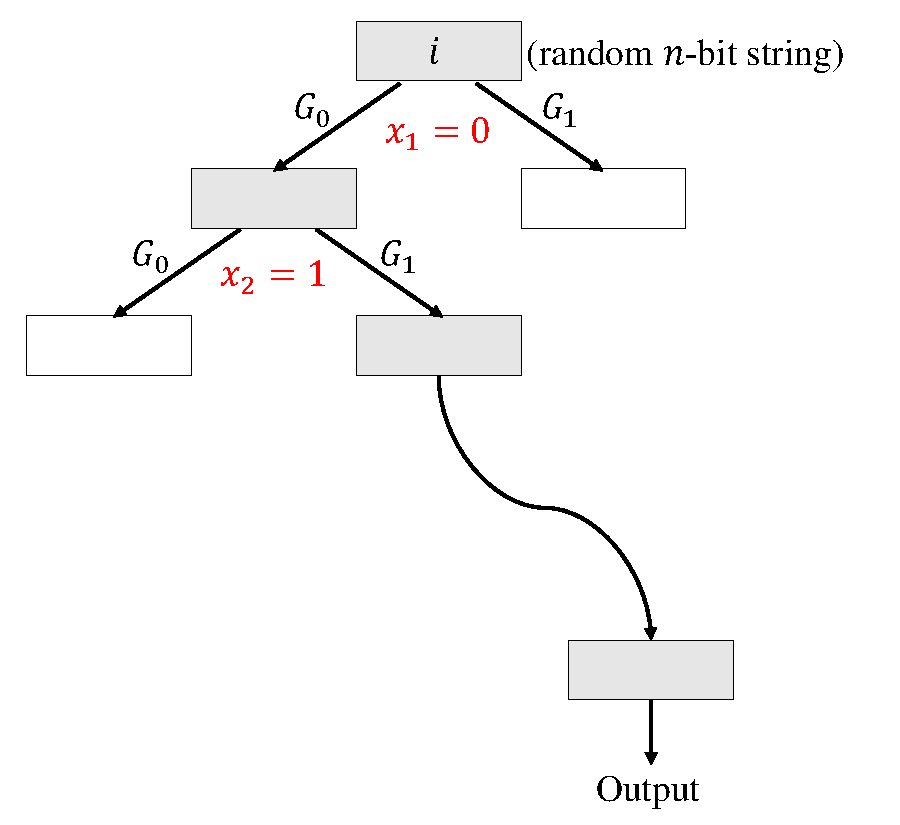
\includegraphics[width=\textwidth]{Old Scribe Notes/binary-tree.pdf}
    \caption{View the construction as a binary tree}
    \label{fig:binary-tree}
\end{marginfigure}

\begin{theorem}\label{theorem:ggm}
The function ensemble $\{F_n\}_{n \in \mathbb{N}}$ constructed above is pseudorandom.
\end{theorem}

\proof
Assume for the sake of contradiction that $\{F_n\}_{n \in \mathbb{N}}$ is not PRG.
Then there exists a non-uniform PPT oracle adversary $\ma$ that can distinguish $\{F_n\}_{n \in \mathbb{N}}$ from $\{R_n\}_{n \in \mathbb{N}}$. Below, via a hybrid argument, we prove that this contradicts the fact that $G$ is a PRG.

Consider the sequence of hybrids $H_i$ for $i \in \{ 0, 1, \cdots, n\}$ where the hybrid $i$ is defined as follows:
\[H_{n,i}^{(K)} (x_1x_2\ldots x_n ):= G_{x_n}(G_{x_{n-1}} (\cdots(G_{x_{i+1}}(K(x_ix_{i-1}\ldots x_1))) \cdots  )), \]
where $K$ is a random function from $\{0,1\}^{i}$ to $\{0,1\}^n$. Intuitively, hybrid $H_i$ corresponds to a binary tree of depth $n$ where the nodes of levels $0$ to $i$ correspond to random values and the nodes at levels $i+1$ to $n$ correspond to pseudorandom values. By inspection, observe that hybrids $H_0$ and $H_n$ are identical to a pseudorandom function and a random function, respectively. There it suffices to prove that hybrids $H_i$ and $H_{i+1}$ are computationally indistinguishable for each $i \in \{ 0, 1, \cdots, n\}$.

We show that $H_{i}$ and $H_{i+1}$ are indistinguishable by considering a sequence of sub-hybrids $H_{i,j}$ for $j \in \{0,\ldots q_{i+1}\}$, where $q_{i+1}$ is the number of the distinct $i-bit$ prefixes of the queries of $\mathcal{A}$.\footnote{Observe that $q_{i+1}$ for each appropriate choice of $i$ is bounded by the running time of $\mathcal{A}$. Hence, this value is bounded by a polynomial in the security parameter.}

We define hybrid $H_{i,j}$ for $j =0$ to be same as hybrid $H_{i}$. Additionally, for $j >0$ hybrid $H_{i,j}$ is defined to be exactly the same as hybrid $H_{i,j-1}$ except the response provided to the attacker for the $j^{th}$ distinct $i-bit$ prefix query of $\mathcal{A}$. Let this prefix be $x^*_n x^*_{n-1} \ldots x^*_{i}$. Note that in hybrid $H_{i,j-1}$ the children of the node $x^*_n x^*_{n-1} \ldots x^*_{i}$ correspond to two pseudorandom values. In hybrid $H_{i,j}$ we replace these two children with random values. By careful inspection, it follows that hybrid $H_{i,q_{i+1}}$ is actually $H_{i+1}$. All we are left to prove is that hybrid $H_{i,j}$ and $H_{i,j+1}$ are indistinguishable for the appropriate choices of $j$ and we prove this below.


Now we are ready to construct an adversary $\mathcal{B}$ that  distinguishes $U_{2n}$ from $G(U_n)$: On input $T \in\{0, 1\}^{2n}$ ($T$ could be either from $U_{2n}$ or $G(U_n)$),
construct a full binary tree of depth $n$ that is exactly the same as $H_{i,j}$ except replacing the children of  $x^*_n x^*_{n-1} \ldots x^*_{i}$ by the value $T$.
Observe that the only difference between $H_{i,j}$ and $H_{i,j+1}$ is that values corresponding to nodes $x_n^*\ldots x_i^* 0$ and $x_n^*\ldots x_i^* 1$ are pseudorandom or random respectively. $\mathcal{B}$ uses the value $T$ to generate these two nodes. Hence success in  distinguishing hybrids $H_{i,j}$ and $H_{i,j+1}$ provides a successful attack for $\mathcal{B}$ in violating security of the pseudorandom generator.
\qed







\section{PRFs from DDH: Naor-Reingold PRF}
We will now describe a PRF function family $F_n: \mathcal{K} \times \{0,1\}^n \rightarrow \mathbb{G}_n$ where DDH is assumed to be hard for  $\{\mathbb{G}_n\}$ and $\mathcal{K}$ is the key space.
The seed for the PRF $F_n$ will be $K =  (h, u_1, \ldots u_n)$, where $u,u_0\ldots u_n$ are sampled uniformly from $|\mathbb{G}_n|$, $g$ is the generator of $\mathbb{G}_n$ and $h = g^u$. 

\[F_n(K,x) = h^{\prod_{i} u_i^{x_i}}\]

Next, we will prove that the function $F_n$ is a pseudo-random function or that $\{F_n\}$ is a pseudo-random function ensemble.\footnote{Here, we require that adversary distinguish the function $F_n$ from a random function from $\{0,1\}^n$ to $\mathbb{G}_n$. Note that the output range of the function is $\mathbb{G}_n$. Note that the distribution of random group elements in $\mathbb{G}_n$ might actually be far from uniformly random strings.}
\begin{lemma}
Assuming the DDH Assumption (see Definition~\ref{def:ddh}) for $\{\mathbb{G}_n\}$ is hard, we have that $\{F_n\}$ is a pseudorandom function ensemble.
\end{lemma}
\begin{proof}
The proof of this lemma is similar to the proof of Theorem~\ref{theorem:ggm}.

Let $R_n^j$ be random function from $\{0,1\}^j \rightarrow \mathbb{G}_n$. Then we want to prove that for all non-uniform PPT adversaries $\mathcal{A}$ we have that:
\[\mu(n) = \left|\Pr[\mathcal{A}^{F_n}(1^n) =1] -  \Pr[\mathcal{A}^{R_n^n}(1^n) =1]\right|\]
is a negligible function. 

For the sake of contradiction, we assume that the function $F_n$ is not pseudorandom. Next, towards a contradiction, we consider a sequence of hybrid functions $F_n^0 \ldots F_n^n$. 
For any $j \in \{0,\ldots n\}$, let $F^j_n((h,u_{j}\ldots u_n),x) = (R_n^j(x_1\ldots x_j))^{\prod_{i=j+1}^n u_i^{x_i}}$, where $R_n^0(\epsilon)$ is the constant function with output $h$. Observe that $F_n^0$ is the same as the function $F_n$ and $F_n^n$ is the same as the function $R_n^n$. Thus, by a hybrid argument, we conclude that there exists $k \in \{0,\ldots n-1\}$, such that 
\[\left|\Pr[\mathcal{A}^{F_n^k}(1^n) =1] -  \Pr[\mathcal{A}^{F_n^{k+1}}(1^n) =1]\right|\]
is a non-negligible function. Now all we are left to show is that this implies an attacker that refutes the DDH assumption. The proof of this claim follows by a sequence of $T$ sub-hybrids, where $T$ is the running time of $\mathcal{A}$. Without loss of generality we assume that $\mathcal{A}$ never makes the same query twice. 

More specifically, we consider a sequence of functions $F_n^{k,t}$ where $t \in \{0,T\}$, $F_n^{k,0}$ is same as $F_n^{k}$ and $F_n^{k,T}$ is same as $F_n^{k+1}$. In particular, we explain how $F_n^{k,t}$ answers queries by $\mathcal{A}$.\footnote{As assumed earlier, keep in mind that $\mathcal{A}$ never makes the same query twice.} Let $x^1, \ldots x^t$ be the first $t$ queries made by $\mathcal{A}$. For any query, $x$ made by $\mathcal{A}$ such that the first $k$ bits of $x$ match the first $k$ bits of one of $x_1, \ldots x_y$ answer as $F_n^{k+1}$ else answer as $F_n^{k}$. Now we can conclude that there exists a $t$ such that $F_n^{k,t}$ and $F_n^{k,t+1}$ are distinguishable with non-negligible probability. 

Finally, we will show that using an adversary that can distinguish between $F_n^{k,t}$ and $F_n^{k,t+1}$ we need to construct an adversary $\mathcal{B}$ that refutes the DDH assumption. We leave construction of this adversary as an exercise.
\end{proof}


\newpage
\section*{Exercises}
\begin{exercise}
\newcommand{\bit}{\{0,1\}}

Prove or disprove: If $f$ is a one-way function, then the following function $B:\bit^*\to\bit$ is a hardconcentrate predicate for $f$. The function $B(x)$ outputs the inner product modulo 2 of the first $\lfloor |x|/2\rfloor$ bits of $x$ and the last $\lfloor |x|/2\rfloor$ bits of $x$.
\end{exercise}

\begin{exercise}
Let $\phi(n)$ denote the first $n$ digits of $\pi = 3.141592653589\ldots$ after the decimal in binary ($\pi$ in its binary notation looks like $11.00100100001111110110101010001000100001\ldots$).

   Prove the following: if one-way functions exist, then there exists a one-way function $f$ such that the function $B:\{0,1\}^* \rightarrow \{0,1\}$ is not a hard concentrate bit of $f$. The function $B(x)$ outputs $\langle x, \phi(|x|)\rangle$, where
    \[\langle a, b\rangle := \sum_{i=1}^n a_i b_i \mod 2\]
    for the bit-representation of $a = {a_1a_2\cdots a_n}$ and $b= {b_1b_2\cdots b_n}$.
\end{exercise}

\begin{exercise}
 If $f: \{0,1\}^{n}\times \{0,1\}^n\rightarrow \{0,1\}^n$  is PRF, then in which of the following cases is $g: \{0,1\}^{n}\times \{0,1\}^n\rightarrow \{0,1\}^n$ also a PRF? \begin{enumerate} \item $g(K,x) = f(K,f(K,x))$ \item $g(K,x) = f(x,f(K,x))$ \item $g(K,x) = f(K,f(x,K))$
    \end{enumerate}
\end{exercise}

\begin{exercise}[Puncturable PRFs.] Puncturable PRFs are PRFs for which a key can be given out such that, it allows evaluation of the PRF on all inputs, except for one designated input.

\newcommand{\negl}{\mathsf{negl}}
\newcommand{\A}{\mathcal{A}}
\newcommand{\F}{F}
\newcommand{\KeyF}{\mathsf{Key}_{\F}}
\newcommand{\PunctureF}{\mathsf{Puncture}_{\F}}
\newcommand{\EvalF}{\mathsf{Eval}_{\F}}


A puncturable pseudo-random function $\F$ is given by a triple of efficient algorithms ($\KeyF$,$\PunctureF$, and $\EvalF$), satisfying the following conditions:
\begin{itemize}
\item[-] \textbf{Functionality preserved under puncturing}: For every $x^*, x \in \{0,1\}^{n}$ such that $x^* \neq x$, we have that:
    $$\Pr[\EvalF(K,x) = \EvalF(K_{x^*},x) : K \gets \KeyF(1^n), K_{x^*} = \PunctureF(K,x^*)] = 1$$
\item[-] \textbf{Pseudorandom at the punctured point}: For every $x^*\in \{0,1\}^n$ we have that for every polysize adversary $\A$ we have that:
    $$|\Pr[\A(K_{x^*}, \EvalF(K,x^*)) = 1] - \Pr[\A(K_{x^*}, \EvalF(K,U_n)) = 1]|= \negl(n)$$
    where $K \gets \KeyF(1^n)$ and $K_S = \PunctureF(K,x^*)$. $U_n$ denotes the uniform distribution over $n$ bits.
\end{itemize}

Prove that: If one-way functions exist, then there exists a puncturable PRF family that maps $n$ bits to $n$ bits. \\ 
\textbf{Hint:} The GGM tree-based construction of PRFs from a length doubling pseudorandom generator (discussed in class) can be adapted to construct a puncturable PRF. Also note that $K$ and $K_{x^*}$ need not be the same length.
\end{exercise}
 \chapter{Private-Key Encryption}   \newcommand{\Gen}{\mathsf{Gen}}
\newcommand{\Sign}{\mathsf{Sign}}
\newcommand{\Verify}{\mathsf{Verify}}
\newcommand{\negl}{\mathsf{negl}}
\newcommand{\abort}{\mathsf{abort}}
\newcommand{\Sampler}{\mathsf{Sampler}}
\newcommand{\Eval}{\mathsf{Eval}}
\renewcommand{\tag}{\mathsf{tag}}
\newcommand{\PRF}{\mathsf{PRF}}

\chapter{Digital Signatures}

In this chapter, we will introduce the notion of a digital signature. At an intuitive level, a digital signature scheme helps providing authenticity of messages and ensuring non-repudiation. We will first define this primitive and then construct what is called as one-time secure digital signature scheme. An one-time digital signature satisfies a weaker security property when compared to digital signatures. We then introduce the concept of collision-resistant hash functions and then use this along with a one-time secure digital signature to give a construction of digital signature scheme.

\section{Definition}

A digital signature scheme is a tuple of three algorithms $(\Gen,\Sign,\Verify)$ with the following syntax:
\begin{enumerate}
\item $\Gen(1^n)\to (vk,sk)$: On input the message length (in unary) $1^n$, $\Gen$ outputs a secret signing key $sk$ and a public verification key $vk$.
\item $\Sign(sk, m) \to \sigma$: On input a secret key $sk$ and a message $m$ of length $n$, the $\Sign$ algorithm outputs a signature $\sigma$.
\item $\Verify(vk, m, \sigma) \to \{0,1\}$: On input the verification key $vk$, a message $m$ and a signature $\sigma$, the $\Verify$ algorithm outputs either $0$ or $1$.
\end{enumerate}

We require that the digital signature to satisfy the following correctness and security properties.\\
\medskip
\noindent\textbf{Correctness.} For the correctness of the scheme, we have that
$\forall m \in \bin^n$,
\[\Pr \left[ (vk,sk) \gets \Gen(1^n), \sigma \leftarrow \Sign(sk,m) : \Verify(vk, m, \sigma) = 1 \right] = 1.\]

\medskip
\noindent\textbf{Security.} Consider the following game between an adversary and a challenger
.

\begin{enumerate}
    \item The challenger first samples $(vk,sk) \gets \Gen(1^n)$. The challenger gives $vk$ to the adversary.
    \item \textbf{Signing Oracle.} The adversary is now given access to a signing oracle. When the adversary gives a query $m$ to the oracle, it gets back $\sigma \gets \Sign(sk,m)$.
    \item \textbf{Forgery.} The adversary outputs a message, signature pair $(m^*,\sigma^*)$ where $m^*$ is different from the queries that adversary has made to the signing oracle.
    \item The adversary wins the game if $\Verify(vk,m^*,\sigma^*) = 1$.
\end{enumerate}
We say that the digital signature scheme is secure if the probability that the adversary wins the game is $\negl(n)$.

\section{One-time Digital Signature}
\label{lampart}
An one-time digital signature has the same syntax and correctness requirement as that of a digital signature scheme except that in the security game the adversary is allowed to call the signing oracle only once (hence the name one-time). We will now give a construction of one-time signature scheme from the assumption that one-way functions exists.

Let $f: \bin^n \rightarrow \bin^n$ be a one-way function.
\begin{itemize}
\item $\Gen(1^n)$: On input the message length (in unary) $1^n$, $\Gen$ does the following:
\begin{enumerate}
    \item Chooses $x_{i,b} \gets \bin^n$ for each $i \in [n]$ and $b \in \bin$.
    \item Output $vk = \left[ \begin{array}{ccc}
f(x_{1,0}) & \ldots & f(x_{n,0}) \\
f(x_{1,1}) & \ldots & f(x_{n,1}) \\
\end{array} \right]$ and $sk = \left[ \begin{array}{ccc}
x_{1,0} & \ldots & x_{n,0} \\
x_{1,1} & \ldots & x_{n,1} \\
\end{array} \right]$
\end{enumerate}
\item $\Sign(sk, m)$: On input a secret key $sk$ and a message $m \in \bin^n$, the $\Sign$ algorithm outputs a signature $\sigma = x_{1,m_1}\|x_{2,m_2}\| \ldots \| x_{n,m_n}$.
\item $\Verify(vk, m, \sigma)$: On input the verification key $vk$, a message $m$ and a signature $\sigma$, the $\Verify$ algorithm does the following:
\begin{enumerate}
    \item Parse $\sigma = x_{1,m_1}\|x_{2,m_2}\| \ldots \| x_{n,m_n}$.
    \item Compute $vk'_{i,m_i} = f(x_{i,m_i})$ for each $i \in [n]$.
    \item Check if for each $i \in [n]$, $vk'_{i,m_i} = vk_{i,m_i}$. If all the checks pass, output 1. Else, output 0.
\end{enumerate}
\end{itemize}

Before we prove any security property, we first observe that this scheme is completely broken if we allow the adversary to ask for two signatures. This is because the adversary can query for the signatures on $0^n$ and $1^n$ respectively and the adversary gets the entire secret key. The adversary can then use this secret key to sign on any message and break the security. 

We will now argue the one-time security of this construction. Let $\adv$ be an adversary who breaks the security of our one-time digital signature scheme with non-negligible probability $\mu(n)$. We will now construct an adversary $\advb$ that breaks the one-wayness of $f$. $\advb$ receives a one-way function challenge $y$ and does the following:
\begin{enumerate}
    \item $\advb$ chooses $i^*$ uniformly at random from $[n]$ and $b^*$ uniformly at random from $\bin$.
    \item It sets $vk_{i^*,b^*} = y$
    \item For all $i \in [n]$ and $b \in \bin$ such that $(i,b) \neq (i^*,b^*)$, $\advb$ samples $x_{i,b} \gets \bin^n$. It computes $vk_{i,b} = f(x_{i,b})$.
    \item It sets $vk = \left[ \begin{array}{ccc}
vk_{1,0} & \ldots& vk_{n,0} \\
vk_{1,1} & \ldots& vk_{n,1} \\
\end{array} \right]$ and sends $vk$ to $\adv$.
\item $\adv$ now asks for a signing query on a message $m$. If $m_{i^*} = b^*$ then $\advb$ aborts and outputs a special symbol $\abort_1$. Otherwise, it uses it knowledge of $x_{i,b}$ for $(i,b) \neq (i^*,b^*)$ to output a signature on $m$.
\item $\adv$ outputs a valid forgery $(m^*,\sigma^*)$. If $m^*_{i^*} = m_{i^*}$ then $\advb$ aborts and outputs a special symbol $\abort_2$. If it does not abort, then it parses $\sigma^*$ as ${1,m_1}\|x_{2,m_2}\| \ldots \| x_{n,m_n}$ and outputs $x_{i^*,b^*}$ as the inverse of $y$.
\end{enumerate}
We first note that conditioned on $\advb$ not outputting $\abort_1$ or $\abort_2$, the probability that $\advb$ outputs a valid preimage of $y$ is $\mu(n)$. Now, probability $\advb$ does not output $\abort_1$ or $\abort_2$ is $1/2n$ (this is because $\abort_1$ is not output with probability $1/2$ and conditioned on not outputting $\abort_1$, $\abort_2$ is not output with probability $1/n$). Thus, $\advb$ outputs a valid preimage with probability $\mu(n)/2n$. This completes the proof of security.

We now try to extend this one-time signature scheme to digital signatures. For this purpose, we will rely on a primitive called as collision-resistant hash functions.

\section{Collision Resistant Hash Functions}

As the name suggests, collision resistant hash function family is a set of hash functions $H$ such that for a function $h$ chosen randomly from the family, it is computationally hard to find two different inputs $x,x'$ such that $h(x) = h(x')$. We now give a formal definition.

\subsection{Definition of a family of CRHF}

A set of function ensembles
\[ \{H_n = \{h_i : D_n \to R_n \}_{i \in I_n} \}_n\]
where $|D_n| < |R_n|$ is a family of collision resistant hash function ensemble if there exists efficient algorithms $(\Sampler,\Eval)$ with the following syntax:
\begin{enumerate}
\item $\Sampler(1^n) \to i:$ On input $1^n$, $\Sampler$ outputs an index $i \in I_n$.
\item $\Eval(i,x) = h_i(x):$ On input $i$ and $x \in D_n$, $\Eval$ algorithm outputs $h_i(x)$. 
\item $\forall$ PPT $\adv$ we have
\[\Pr[i \gets \Sampler(1^n), (x,x') \gets \adv(1^n,i) : h_i(x) = h_i(x') \wedge x \neq x'] \leq \negl(n)\]
\end{enumerate}


\subsection{Collision Resistant Hash functions from Discrete Log}
We will now give a construction of collision resistant hash functions from the discrete log assumption. We first recall the discrete log assumption:
\begin{definition}[Discrete-Log Assumption]
We say that the discrete-log assumption holds for the group ensemble $\mathcal{G} =\{ \mathbb{G}_n\}_{n \in \mathbb{N}}$, if for every non-uniform PPT algorithm $\mathcal{A}$ we have that
\[\mu_\mathcal{A}(n) := \Pr_{x \leftarrow |G_n|}[\mathcal{A}(g,g^x) = x]\]
is a negligible function.
\end{definition}

We now give a construction of collision resistant hash functions.  

\begin{itemize}
\item $\Sampler(1^n):$ On input $1^n$, the sampler does the following:
\begin{enumerate}
    \item It chooses $x \gets |\mathbb{G}_n|$.
    \item It computes $h = g^x$.
    \item It outputs $(g,h)$.

\end{enumerate}
\item $\Eval((g,h),(r,s)):$ On input $(g,h)$ and two elements $(r,s) \in |\mathbb{G}_n|$, $\Eval$ outputs $g^rh^s$.
\end{itemize}

We now argue that this construction is collision resistant. Assume for the sake of contradiction that an adversary gives a collision $(r_1,s_1) \neq (r_2,s_2)$. We will now use this to compute the discrete logarithm of $h$. We first observe that:
\begin{eqnarray*}
r_1+xs_1 &=& r_2 + xs_2\\
(r_1 - r_2) &=& x(s_2 - s_1)
\end{eqnarray*}
We infer that $s_2 \neq s_1$. Otherwise, we get that $r_1 = r_2$ and hence, $(r_1,s_1) = (r_2,s_2)$. Thus, we can compute $x = \frac{r_1-r_2}{s_1 - s_2}$ and hence the discrete logarithm of $h$ is computable.


\section{Multiple-Message Digital Signature}

We now explain how to combine collision-resistant hash functions and one-time signatures to get a signature scheme for multiple messages. We first construct an intermediate primitive wherein we will still have the same security property as that of one-time signature but we would be able to sign messages longer than the length of the public-key.\footnote{Note that in the one-time signature scheme that we constructed earlier, the length of message that can be signed is same as the length of the public-key.}


\subsection{One-time Signature Scheme for Long Messages}
We first observe that the CRHF family $H$ that we constructed earlier compresses $2n$ bits to $n$ bits (also called as 2-1 CRHF). We will now give an extension that compresses an arbitrary long string to $n$ bits using a 2-1 CRHF.
\paragraph{Merkle-Damgard CRHF.} The sampler for this CRHF is same as that of 2-1 CRHF. Let $h$ be the sampled hash function. To hash a string $x$, we do the following. Let $x$ be a string of length $m$ where $m$ is an arbitrary polynomial in $n$. We will assume that $m = kn$ (for some $k$) or otherwise, we can pad $x$ to this length. We will partition  the string $x$ into $k$ blocks of length $n$ each. For simplicity, we will assume that $k$ is a perfect power of $2$ or we will again pad $x$ appropriately. We will view these $k$-blocks as the leaves of a complete binary tree of depth $\ell = \log_2 k$. Each intermediate node is associated with a bit string $y$ of length at most $\ell$ and the root is associated with the empty string. We will assign a $\tag \in \bin^n$ to each node in the tree. The $i$-th leaf is assigned $\tag_i$ equal to the $i$-block of the string $x$. Each intermediate node $y$ is assigned a $\tag_y = h(\tag_{y\|0}\| \tag_{y \| 1})$. The output of the hash function is set to be the $\tag$ value of the root. Notice that if there is a collision for this CRHF then there are exists one intermediate node $y$ such that for two different values $\tag_{y\|0},\tag_{y\|1}$ and $\tag'_{y\|0},\tag'_{y\|1}$ we have, $h(\tag_{y\|0},\tag_{y\|1}) = \tag'_{y\|0},\tag'_{y\|1}$. This implies that there is a collision for $h$. 

\paragraph{Construction.} We will now use the Merkle-Damgard CRHF and the one-time signature scheme that we constructed earlier to get a one-time signature scheme for signing longer messages. The main idea is simple: we will sample a $(sk,vk)$ for signing $n$-bit messages and to sign a longer message, we will first hash it using the Merkle-Damgard hash function to $n$-bits and then sign on the hash value. The security of the construction follows directly from the security of the one-time signature scheme since the CRHF is collision-resistant. 

\subsection{Signature Scheme for Multiple Messages}
We will now describe the construction of signature scheme for multiple messages. Let $(\Gen',\Sign',\Verify')$ be a one-time signature scheme for signing longer messages. 
\begin{enumerate}
    \item $\Gen(1^n):$ Run $\Gen'(1^n)$ using to obtain $sk,vk$. Sample a PRF key $K$. The signing key is $(sk,K)$ and the verification key is $vk$.
    \item $\Sign((sk,K),m):$ To sign a message $m$, do the following:
    \begin{enumerate}
        \item Parse $m$ as $m_1m_2\ldots m_{\ell}$ where each $m_i \in \bin$.
        \item Set $sk_0 = sk$ and $m_0 = \epsilon$ (where $\epsilon$ is the empty string).
        \item For each $i \in [\ell]$ do:
        \begin{enumerate}
            \item Evaluate $\PRF(m_1\|\ldots\|m_{i-1}\|0)$ and $\PRF(m_1\|\ldots\|m_{i-1}\|1)$ to obtain $r_0$ and $r_1$ respectively. Run $\Gen'(1^n)$ using $r_0$ and $r_1$ as the randomness to obtain $(sk_{i,0},vk_{i,1})$ and $(sk_{i,1},vk_{i,1})$.
            \item Set $\sigma_i = \Sign(sk_{i-1,m_{i-1}},vk_{i,0}\|vk_{i,1})$
            \item If $i = \ell$, then set $\sigma_{\ell+1} = \Sign(sk_{i,m_i},m)$.

        \end{enumerate}
        \item Output $\sigma = (\sigma_1,\ldots,\sigma_{\ell+1})$ along with all the verification keys as the signature.
    \end{enumerate}
    \item $\Verify(vk,\sigma,m)$: Check if all the signatures in $\sigma$ are valid.
\end{enumerate}

To prove security, we will first use the security of the PRF to replace the outputs with random strings. We will then use the security of the one-time signature scheme to argue that the adversary cannot mount an existential forgery.

\section*{Exercises}
\begin{exercise}
\textbf{Digital signature schemes can be made deterministic.} Given a digital signature scheme $(\mathsf{Gen}, \mathsf{Sign}, \mathsf{Verify})$ for which $\mathsf{Sign}$ is probabilistic, provide a construction of a digital signature scheme $(\mathsf{Gen}', \mathsf{Sign}', \mathsf{Verify}')$ where $\mathsf{Sign}'$ is deterministic.
\end{exercise}





\backmatter

\bibliography{cryptobib/abbrev0,cryptobib/crypto}
\bibliographystyle{plainnat}




\end{document}
